%% HARNESS-Review — supplementary material (acmart, standalone root).
%% Same class, options, packages and bibliography as main.tex; compile on its own:
%%   cd paper && latexmk -pdf -interaction=nonstopmode supplement.tex
%% Cross-references into the main paper cannot resolve in a standalone build, so the supplement
%% sections point into the main paper in prose ("\S4") and use \ref only for their own labels.
\documentclass[manuscript,screen,review]{acmart}
\usepackage{booktabs}
\usepackage{graphicx}
\usepackage{xcolor}
%% The RQ3 macros the main paper uses; the artefact map (S5) cites the generated values through them.
% RQ3 prose macros (text-mode safe; *Pct macros are bare numbers)
% GENERATED by scripts/make_rq3_tables.py - do not edit; re-run the script instead.
% sources (mtime, UTC):
%   data/analysis/ablation_summary_corpus.json  (2026-09-28T13:53:56Z)
%   data/analysis/ablation_pooled_corpus.csv  (2026-09-28T13:53:56Z)
%   data/analysis/ablation_credible_corpus.csv  (2026-09-28T13:53:56Z)
%   data/analysis/ablation_bias_corpus.csv  (2026-09-28T13:53:56Z)
%   data/analysis/ablation_contrasts_corpus.csv  (2026-09-28T13:53:56Z)
%   data/analysis/ablation_coverage_summary.json  (2026-09-25T16:01:11Z)
%   data/analysis/ablation_coverage_summary_corpus.json  (2026-09-28T13:53:57Z)
%   schema/dimensions.json  (2026-09-25T14:21:14Z)
%   paper/tables/outcomes_summary.json  (2026-09-25T15:27:23Z)
%   data/results.csv  (2026-09-24T23:51:08Z)
%   data/systems.json  (2026-09-25T10:17:13Z)
%   data/analysis/corpus_ablation_rows.csv  (live; rows of the pooled snapshot's papers only)
%   data/analysis/corpus_ablation_outcomes.csv  (live; rows of the pooled snapshot's papers only)
% generated: 2026-09-28T13:53:57Z
% papers the corpus-wide harvest has read (snapshot pooled)
\newcommand{\rqCorpusPapersExtracted}{2{,}824}
% corpus-harvest papers contributing >=1 pooled contrast (after de-duplication)
\newcommand{\rqCorpusPapersWithContrast}{1{,}264}
% corpus-harvest contrasts pooled (after de-duplication against the coded set)
\newcommand{\rqCorpusContrasts}{5{,}928}
% coded-set harvest contrasts
\newcommand{\rqCodedContrasts}{75}
% coded-set harvest papers
\newcommand{\rqCodedPapers}{42}
% all contrasts pooled, coded-set + corpus
\newcommand{\rqTotalContrasts}{6{,}003}
% distinct papers behind them
\newcommand{\rqTotalPapers}{1{,}278}
% corpus contrasts dropped as already in the coded-set harvest
\newcommand{\rqCorpusDuplicatesDropped}{48}
% dimensions pooled (>= rqMinPapers papers)
\newcommand{\rqPoolableDims}{22}
% papers needed to pool a dimension
\newcommand{\rqMinPapers}{3}
% bare number: % of contrasts favouring the component, coded-set + corpus, over the pooled (bias-diagnosed) dimensions, contrast-weighted
\newcommand{\rqSignSharePct}{90.0}
% pooled dimensions whose 95% prediction interval includes zero
\newcommand{\rqPIIncludesZeroCount}{22}
% pooled dimensions whose prediction interval excludes zero
\newcommand{\rqPIExcludesZeroDims}{none}
% lower prediction-interval bound of each of those dimensions
\newcommand{\rqPIExcludesZeroLower}{none}
% pooled dimensions surviving the bias discount on the z interval
\newcommand{\rqDiscountSurviveZ}{14}
% ... on the Hartung-Knapp interval
\newcommand{\rqDiscountSurviveHK}{14}
% min to max DL pooled effect over the dimensions surviving on z
\newcommand{\rqEffectRangeSurviving}{\ensuremath{+0.114} to \ensuremath{+0.259}}
% first to third quartile of those effects (inclusive quartiles)
\newcommand{\rqEffectIQRSurviving}{\ensuremath{+0.159} to \ensuremath{+0.188}}
% bare number: median per-dimension publication-bias discount, %
\newcommand{\rqMedianDiscountPct}{49.5}
% dimensions with Egger p < 0.1, intercept sign in parentheses
\newcommand{\rqEggerFlaggedDims}{observation\_format (\ensuremath{-}), tool\_count (\ensuremath{-}), planning\_granularity (\ensuremath{-}), long\_term\_memory (\ensuremath{-}), self\_verification (\ensuremath{-}), termination\_condition (\ensuremath{+})}
% focal dimension: papers
\newcommand{\rqSVPapers}{525}
% focal dimension: contrasts
\newcommand{\rqSVContrasts}{1{,}687}
% focal dimension: DL pooled effect
\newcommand{\rqSVPooled}{\ensuremath{+0.152}}
% focal dimension: discounted effect
\newcommand{\rqSVDiscounted}{\ensuremath{+0.152}}
% focal dimension: 95% prediction interval, with brackets
\newcommand{\rqSVPI}{\ensuremath{[-0.798, +1.101]}}
% focal dimension: 95% z confidence interval, with brackets
\newcommand{\rqSVCIz}{\ensuremath{[+0.109, +0.194]}}
% focal dimension: 95% Hartung-Knapp interval, with brackets
\newcommand{\rqSVCIHK}{\ensuremath{[+0.128, +0.175]}}
% Spearman rho, layer silence vs corpus-wide ablation density
\newcommand{\rqCoverageRho}{\ensuremath{-0.738}}
% its exact one-sided permutation p
\newcommand{\rqCoverageP}{0.023}
% the same rho on the coded-set harvest only
\newcommand{\rqCodedCoverageRho}{\ensuremath{-0.854}}
% its exact p
\newcommand{\rqCodedCoverageP}{0.0065}
% ablatable dimensions with no contrast at all
\newcommand{\rqZeroDimCount}{7}
% ablatable dimensions (layers A-H)
\newcommand{\rqAblatableDimCount}{31}
% those dimensions
\newcommand{\rqZeroDimList}{cost controls (F2), evaluation hooks (H3), execution isolation (G1), filesystem access (G2), network policy (G3), permission model (G4) and replayability (H2)}
% layers with no ablated dimension ('empty' if none)
\newcommand{\rqZeroLayerList}{G (sandbox and environment)}
% every F/G/H dimension with >=1 contrast: key (papers/contrasts), corpus-wide
\newcommand{\rqFGHPaperCounts}{termination\_condition (9/28), timeouts (1/1), tracing (4/10), guardrails (21/37)}
% noun phrase: share of each prefilter tier the harvest has read
\newcommand{\rqHarvestTierCoverage}{96.7\% of the top-signal tier and 90.1\% of the second}
% papers in the top-signal tier
\newcommand{\rqHarvestTopTierPapers}{899}
% papers in the second tier
\newcommand{\rqHarvestSecondTierPapers}{2{,}170}
% date of the harvest snapshot pooled
\newcommand{\rqHarvestDate}{28 September 2026}
% contrasts on the pooled dimensions: the denominator of rqSignSharePct
\newcommand{\rqSignDenom}{6{,}001}
% of those, contrasts whose metric names its direction (higher / lower is better)
\newcommand{\rqPolarityStatedN}{4{,}080}
% of those, favouring the component
\newcommand{\rqPolarityStatedFavour}{3{,}701}
% bare number: their share favouring the component, %
\newcommand{\rqPolarityStatedFavourPct}{90.7}
% contrasts whose metric names no direction: higher-is-better assumed
\newcommand{\rqPolarityAssumedN}{1{,}921}
% of those, favouring the component
\newcommand{\rqPolarityAssumedFavour}{1{,}700}
% bare number: their share favouring the component, %
\newcommand{\rqPolarityAssumedFavourPct}{88.5}
% contrasts whose variance is a flat assumed relative SE, not a binomial reconstruction
\newcommand{\rqVarAssumedN}{2{,}857}
% Spearman rho, silence vs density, with the seven classification rules undone
\newcommand{\rqPreRuleRho}{\ensuremath{-0.738}}
% its exact one-sided permutation p
\newcommand{\rqPreRuleP}{0.023}
% sandbox-layer (G) contrasts before the rules; after them there are none
\newcommand{\rqPreRuleGContrasts}{20}
% of those, reassigned by a rule to the dimension the removal takes away
\newcommand{\rqPreRuleGRemapped}{13}
% of those, dropped by a rule: delta_metric_as_score 2, scores_not_separable 4, tool_gating_is_tool_interface 1
\newcommand{\rqPreRuleGDropped}{7}
% rows the label-contradicts-orientation rule dropped, on pooled dimensions
\newcommand{\rqDCLDropped}{169}
% of those, rows that do not favour the component as the extraction stage oriented them
\newcommand{\rqDCLAgainst}{71}
% bare number: the sign share had those rows been kept as the extraction oriented them
\newcommand{\rqSignShareWithDCLPct}{89.1}
% headline keys whose reference side is only recurring baseline harnesses
\newcommand{\rqXPBaselineKeys}{7}
% the headline's remaining keys
\newcommand{\rqXPOtherKeys}{11}
% the headline effect on those keys, within-key sd
\newcommand{\rqXPOtherEffect}{\ensuremath{+0.57}}
% its 95% bootstrap interval over keys, with brackets
\newcommand{\rqXPOtherCI}{\ensuremath{[-0.19, +1.23]}}
% its two-sided within-key permutation p
\newcommand{\rqXPOtherP}{0.129}

\graphicspath{{figures/}}

% Allow long artefact paths in the artefact map to break after underscores and hyphens as well.
\makeatletter
\g@addto@macro\UrlBreaks{\do\_\do\-}
\makeatother

% Supplement numbering: sections S1--S6, tables Table S1, S2, ...
\renewcommand{\thesection}{S\arabic{section}}
\renewcommand{\thetable}{S\arabic{table}}
\renewcommand{\thefigure}{S\arabic{figure}}

\acmJournal{CSUR}
\citestyle{acmauthoryear}
\settopmatter{printacmref=false}

\title[Supplementary material: The Anatomy of Agent Harnesses]{Supplementary material for: The Anatomy of Agent Harnesses: A Systematic Review, Unified Taxonomy, and Coded Dataset (HARNESS-DB) of LLM Agent Scaffolding, 2022--2026}

\author{Bhaskar Gurram}
\email{gurrambhaskar.ai@gmail.com}
\affiliation{%
  \institution{Independent researcher}
  \country{USA}}

\begin{document}

\maketitle

This document is the supplementary material to the main paper. It carries the material a reader
needs to check or reuse the review but not to follow its argument, and it is cited from the main
paper by section: a section sign (\S) in what follows refers to a section of the main paper, and
S1--S6 to the sections below.
S1 is the coding sheet and coding manual: all 38 dimensions in nine layers with their permitted values,
the general coding rules, and two systems coded end to end.
S2 is the full log of the eleven protocol amendments accepted at OSF, each with its date, the protocol
section it changes, its reason, and whether it was filed before the stage it changes, together with the
twelfth and its dated revision (12a), both filed and pending acceptance.
S3 is the PRISMA 2020 checklist, mapping each of the 27 items to the place it is reported.
S4 describes the released dataset: what is released and under which licence, the counts that let a
reader check the release against the paper, a 12-system extract, and the per-dimension reliability
tables.
S5 is the artefact map, which ties every quantity reported in the paper to the artefact in the
replication package that carries it and the script that regenerates it.
S6 holds material moved from the main paper for its page budget: the synthesis-estimator table, the
full twelve-item reporting checklist, and four landscape figures (every value of every dimension,
per-dimension under-reporting, entropy trajectories, and the pair-by-pair association change).

% S1 — coding sheet and manual (maintained with the main-paper sections; guarded so this root
% compiles while that file is being rewritten).
\IfFileExists{sections/A1_coding_sheet.tex}{%
  \section{Coding sheet and coding manual}
\label{app:coding}

This supplement is the coding frame itself: all 38 dimensions in nine layers, each with its complete
permitted value set, reproduced from the frozen schema (v1.0.0) in the replication package. The main
text argues for the frame (\S5) and describes how it was applied (\S4);
neither argument is restated here. The schema was frozen on 2026-09-23, and no dimension has been added,
removed, renamed, or re-valued since the initial draft. Every table in this supplement is generated from
the schema by a script, so it cannot drift from what was coded.

The manuscript preamble loads \texttt{booktabs} and \texttt{graphicx} but not \texttt{longtable}, and a
section file cannot load a package, so the frame is given as nine per-layer tables
(Tables~\ref{tab:coding-A}--\ref{tab:coding-M}). A dimension is \emph{single} when one value is recorded
and \emph{multi} when every applicable value is recorded; 15 of the 38 are multi. Four dimensions
(\texttt{tool\_count}, \texttt{first\_release\_date}, \texttt{pinned\_version}, \texttt{stars}) carry a
scalar type instead of a value set. Each layer's table is preceded by the judgment call that layer
raised, illustrated by the two systems coded end to end in the manual,
SWE-agent v1.1.0~\citep{yang2024sweagent} and OpenHands v1.16.0~\citep{wang2024openhands}
(Section~\ref{subsec:coding-examples}).

\subsection{Coding sheet and judgment calls by layer}
\label{subsec:coding-sheet}

\paragraph{Layer A: context assembly.}\label{subsec:layer-a}
Layer A governs what the model sees at each step. A3 and A4 are multi-valued because compaction
mechanisms and observation modalities stack in one system, while a prompt-production strategy and a
context strategy do not. The judgment call on A1 is where a template stops. Variables rendered once per
run are \texttt{templated}; conditional sections, runtime-loaded files, or per-step recomposition are
\texttt{dynamically\_composed}; a paper that says only ``we prompt the model with'' is \texttt{static}
at low confidence. On A2, \texttt{mixed} is coded only when the default configuration both injects
context and lets the model navigate. The worked systems split on both dimensions. SWE-agent renders one
Jinja template per run and prunes tool output only: A1 \texttt{templated}, A3
\texttt{[tool\_output\_pruning]}. OpenHands composes a static tier from a section registry with a
dynamic tier from its agent context, and runs a summarizing condenser by default: A1
\texttt{dynamically\_composed}, A3 \texttt{[summarize, tool\_output\_pruning]}.

\begin{table}[htbp]
\caption{Layer \texttt{A}, Context assembly: 4 dimensions, with ids, names, keys, types and value
sets verbatim from the frozen schema (v1.0.0).}
\label{tab:coding-A}
\footnotesize
\begin{tabular}{@{}l p{0.20\linewidth} p{0.22\linewidth} l p{0.33\linewidth}@{}}
\toprule
ID & Dimension and key & What it records & Type & Permitted values \tabularnewline
\midrule
\texttt{A1} & \raggedright System-prompt style \newline \texttt{system\_prompt\_style} & \raggedright how the system prompt that opens every model call is produced & enum, single & \raggedright \texttt{static}, \texttt{templated}, \texttt{dynamically\_composed}, \texttt{model\_generated} \tabularnewline
\texttt{A2} & \raggedright Repo/environment context strategy \newline \texttt{env\_context\_strategy} & \raggedright how the model is given knowledge of the repository or environment & enum, single & \raggedright \texttt{none}, \texttt{file\_tree\_summary}, \texttt{retrieval\_bm25}, \texttt{embedding\_rag}, \texttt{agent\_driven\_navigation}, \texttt{mixed} \tabularnewline
\texttt{A3} & \raggedright Context compaction \newline \texttt{context\_compaction} & \raggedright mechanisms that shrink the history sent to the model & enum, multi & \raggedright \texttt{none}, \texttt{truncate\_oldest}, \texttt{summarize}, \texttt{tool\_output\_pruning}, \texttt{structured\_checkpoint}, \texttt{model\_native} \tabularnewline
\texttt{A4} & \raggedright Observation formatting \newline \texttt{observation\_format} & \raggedright the format in which tool results are presented to the model & enum, multi & \raggedright \texttt{raw\_text}, \texttt{structured\_json}, \texttt{screenshots}, \texttt{a11y\_tree}, \texttt{set\_of\_marks} \tabularnewline
\bottomrule
\end{tabular}
\end{table}

\paragraph{Layer B: tool interface.}\label{subsec:layer-b}
Layer B governs how actions are declared to the model and parsed back out of its output. Four of its
five dimensions are multi-valued, because harnesses ship several parsers, edit commands, and schema
sources at once; the exception, B2, is an integer and carries no value set. B2 is the layer's hardest
judgment call, because ``how many tools'' has no natural answer. The rule counts one entry per function
schema sent with the model call, and counts a built-in shell tool once regardless of what it can run. It
expands a toolset into its tools and counts built-ins attached to every agent, but excludes tools
injected by an MCP server or by the environment, and the maximal shipped configuration goes in the note.
SWE-agent is therefore \texttt{3} at the default against 17 tool definitions shipped across 13 bundles,
and OpenHands \texttt{5} against 19 once the 14-tool browser toolset is injected where Chromium exists.
Both counts are defensible and they are not the same measurement, which is why the counting rule rather
than the count is the taxonomy's content.

\begin{table}[htbp]
\caption{Layer \texttt{B}, Tool interface: 5 dimensions, with ids, names, keys, types and value
sets verbatim from the frozen schema (v1.0.0).}
\label{tab:coding-B}
\footnotesize
\begin{tabular}{@{}l p{0.20\linewidth} p{0.22\linewidth} l p{0.33\linewidth}@{}}
\toprule
ID & Dimension and key & What it records & Type & Permitted values \tabularnewline
\midrule
\texttt{B1} & \raggedright Tool-call format \newline \texttt{tool\_call\_format} & \raggedright the syntax by which the model requests an action & enum, multi & \raggedright \texttt{native\_function\_calling}, \texttt{json\_in\_text}, \texttt{xml\_tags}, \texttt{code\_as\_action}, \texttt{shell\_only}, \texttt{cli\_flags} \tabularnewline
\texttt{B2} & \raggedright Tool count at pinned version \newline \texttt{tool\_count} & \raggedright distinct tool definitions exposed to the model in the default configuration & integer, single & \raggedright no enumerated set (integer) \tabularnewline
\texttt{B3} & \raggedright Edit primitive \newline \texttt{edit\_primitive} & \raggedright how the model expresses a file modification & enum, multi & \raggedright \texttt{none}, \texttt{whole\_file\_rewrite}, \texttt{search\_replace}, \texttt{unified\_diff}, \texttt{line\_range\_edit}, \texttt{ast\_aware} \tabularnewline
\texttt{B4} & \raggedright Tool schema source \newline \texttt{tool\_schema\_source} & \raggedright where the tool schema shown to the model comes from & enum, multi & \raggedright \texttt{hand\_written}, \texttt{auto\_generated}, \texttt{mcp}, \texttt{openapi} \tabularnewline
\texttt{B5} & \raggedright Protocol standardization \newline \texttt{protocol\_standardization} & \raggedright standard agent or tool protocols the harness speaks & enum, multi & \raggedright \texttt{none}, \texttt{mcp}, \texttt{a2a}, \texttt{other} \tabularnewline
\bottomrule
\end{tabular}
\end{table}

\paragraph{Layer C: control loop.}\label{subsec:layer-c}
Layer C governs what happens between model calls: loop shape, plan representation, agent count,
hand-offs, and the points where a human can intervene. C1 and C5 are multi-valued because a harness can
run a ReAct loop inside an event stream and can gate at more than one point. The judgment call across the
whole layer is default versus capability. Decision rule~4 codes the shipped default and records
reachable alternatives in the note, so OpenHands, which ships a delegate tool but sets
\texttt{enable\_sub\_agents=False}, is C3 \texttt{single} and C4 \texttt{none}, with
\texttt{orchestrator\_workers} and \texttt{subagent\_spawn} named as opt-in. C2 draws a related line: a
structured plan the harness writes and re-reads across steps is \texttt{explicit\_plan\_object}, as in
OpenHands' task tracker, while a numbered recipe in the prompt is \texttt{implicit}, as in SWE-agent.

\begin{table}[htbp]
\caption{Layer \texttt{C}, Control loop: 5 dimensions, with ids, names, keys, types and value
sets verbatim from the frozen schema (v1.0.0).}
\label{tab:coding-C}
\footnotesize
\begin{tabular}{@{}l p{0.20\linewidth} p{0.22\linewidth} l p{0.33\linewidth}@{}}
\toprule
ID & Dimension and key & What it records & Type & Permitted values \tabularnewline
\midrule
\texttt{C1} & \raggedright Loop primitive(s) \newline \texttt{loop\_primitives} & \raggedright the control-flow patterns that drive model calls and actions & enum, multi & \raggedright \texttt{react}, \texttt{plan\_execute}, \texttt{generate\_test\_repair}, \texttt{multi\_attempt}, \texttt{tree\_search}, \texttt{event\_driven}, \texttt{fixed\_pipeline} \tabularnewline
\texttt{C2} & \raggedright Planning granularity \newline \texttt{planning\_granularity} & \raggedright whether and how a plan is represented & enum, single & \raggedright \texttt{none}, \texttt{implicit}, \texttt{explicit\_plan\_object}, \texttt{hierarchical} \tabularnewline
\texttt{C3} & \raggedright Multi-agent topology \newline \texttt{multi\_agent\_topology} & \raggedright the arrangement of agents in the default configuration & enum, single & \raggedright \texttt{single}, \texttt{orchestrator\_workers}, \texttt{peer}, \texttt{hierarchical}, \texttt{debate}, \texttt{pipeline} \tabularnewline
\texttt{C4} & \raggedright Delegation mechanism \newline \texttt{delegation\_mechanism} & \raggedright how work is handed to another agent, if at all & enum, single & \raggedright \texttt{none}, \texttt{subagent\_spawn}, \texttt{role\_handoff}, \texttt{message\_bus} \tabularnewline
\texttt{C5} & \raggedright Human-in-the-loop points \newline \texttt{human\_in\_loop} & \raggedright the points at which a human can gate or steer the run & enum, multi & \raggedright \texttt{none}, \texttt{on\_permission}, \texttt{on\_plan}, \texttt{on\_completion}, \texttt{configurable} \tabularnewline
\bottomrule
\end{tabular}
\end{table}

\paragraph{Layer D: memory and state.}\label{subsec:layer-d}
Layer D separates what outlives a model call from what outlives a run: working state inside a run (D1),
information carried between runs (D2), and whether an interrupted run can continue (D3). Only D2 is
multi-valued, because a harness can keep file notes and a skill library at once. The judgment call sits
on D3, where a trajectory file is not a checkpoint. Both \texttt{checkpoint} and \texttt{full\_resume}
require a code path that reads saved state back into a running agent. SWE-agent writes a per-step
trajectory but offers no path to resume from it, so it is \texttt{none} with the trajectory noted.
OpenHands reloads a conversation from a state file and an event directory, so it is
\texttt{full\_resume}. D2 excludes static few-shot demonstrations chosen in configuration, which are
prompt content rather than memory.

\begin{table}[htbp]
\caption{Layer \texttt{D}, Memory and state: 3 dimensions, with ids, names, keys, types and value
sets verbatim from the frozen schema (v1.0.0).}
\label{tab:coding-D}
\footnotesize
\begin{tabular}{@{}l p{0.20\linewidth} p{0.22\linewidth} l p{0.33\linewidth}@{}}
\toprule
ID & Dimension and key & What it records & Type & Permitted values \tabularnewline
\midrule
\texttt{D1} & \raggedright Short-term state \newline \texttt{short\_term\_state} & \raggedright what the harness keeps as working state within a run & enum, single & \raggedright \texttt{conversation\_only}, \texttt{scratchpad}, \texttt{structured\_task\_state} \tabularnewline
\texttt{D2} & \raggedright Long-term memory \newline \texttt{long\_term\_memory} & \raggedright information persisted across runs and re-injected & enum, multi & \raggedright \texttt{none}, \texttt{file\_notes}, \texttt{vector\_store}, \texttt{skill\_library}, \texttt{episodic\_db} \tabularnewline
\texttt{D3} & \raggedright State persistence across runs \newline \texttt{state\_persistence} & \raggedright whether an interrupted run can be continued & enum, single & \raggedright \texttt{none}, \texttt{checkpoint}, \texttt{full\_resume} \tabularnewline
\bottomrule
\end{tabular}
\end{table}

\paragraph{Layer E: verification and repair.}\label{subsec:layer-e}
Layer E records checks the harness enforces, not checks the model could choose to perform. E1 is
multi-valued because linting, test execution, and a judge model coexist, while a retry policy and a
rollback mechanism are one choice each. The enforcement boundary is the layer's main judgment call: if
the model may run tests through a shell but the harness neither runs them nor reads their result,
\texttt{test\_execution} is not coded. E3 shows the closest-value rule at work. Both worked systems
expose a model-invocable per-file \texttt{undo\_edit} backed by saved copies, which is not a filesystem
or container snapshot; both are coded \texttt{snapshot} with the mismatch written into the note and
listed among the ambiguities (Table~\ref{tab:ambiguities-full}).

\begin{table}[htbp]
\caption{Layer \texttt{E}, Verification and repair: 3 dimensions, with ids, names, keys, types and value
sets verbatim from the frozen schema (v1.0.0).}
\label{tab:coding-E}
\footnotesize
\begin{tabular}{@{}l p{0.20\linewidth} p{0.22\linewidth} l p{0.33\linewidth}@{}}
\toprule
ID & Dimension and key & What it records & Type & Permitted values \tabularnewline
\midrule
\texttt{E1} & \raggedright Self-verification \newline \texttt{self\_verification} & \raggedright checks the harness applies, or prompts for, on the agent's work & enum, multi & \raggedright \texttt{none}, \texttt{self\_critique}, \texttt{test\_execution}, \texttt{linters\_typecheck}, \texttt{llm\_judge}, \texttt{formal} \tabularnewline
\texttt{E2} & \raggedright Retry policy \newline \texttt{retry\_policy} & \raggedright task-level retry behavior after a failed or rejected attempt & enum, single & \raggedright \texttt{none}, \texttt{fixed\_n}, \texttt{until\_pass}, \texttt{adaptive} \tabularnewline
\texttt{E3} & \raggedright Rollback / undo \newline \texttt{rollback} & \raggedright the mechanism that reverts changes made during the run & enum, single & \raggedright \texttt{none}, \texttt{git\_based}, \texttt{snapshot} \tabularnewline
\bottomrule
\end{tabular}
\end{table}

\paragraph{Layer F: budget and termination.}\label{subsec:layer-f}
Layer F records what bounds a run. Termination conditions, cost controls, and timeouts each admit a
set, because bounds accumulate rather than exclude one another. A condition counts only if it stops the
loop rather than merely logging, and an off-by-default cap counts when a configuration field exists,
with the default stated in the note. The layer's ambiguity is what \texttt{max\_steps} and
\texttt{max\_tokens} mean in practice: SWE-agent caps API calls rather than agent steps, and exits on
context-window overflow rather than on a token budget. F3 is narrower than it looks, because iteration
caps are not timeouts. SWE-agent is \texttt{[per\_tool, per\_run]}, where the per-run limit counts
cumulative command execution time and not wall-clock; OpenHands is \texttt{[per\_tool]}, with the
absence of a run-level timeout evidenced by the search that found none.

\begin{table}[htbp]
\caption{Layer \texttt{F}, Budget and termination: 3 dimensions, with ids, names, keys, types and value
sets verbatim from the frozen schema (v1.0.0).}
\label{tab:coding-F}
\footnotesize
\begin{tabular}{@{}l p{0.20\linewidth} p{0.22\linewidth} l p{0.33\linewidth}@{}}
\toprule
ID & Dimension and key & What it records & Type & Permitted values \tabularnewline
\midrule
\texttt{F1} & \raggedright Termination condition \newline \texttt{termination\_condition} & \raggedright the conditions that end a run & enum, multi & \raggedright \texttt{model\_declared}, \texttt{max\_steps}, \texttt{max\_tokens}, \texttt{cost\_cap}, \texttt{test\_pass}, \texttt{stall\_detection} \tabularnewline
\texttt{F2} & \raggedright Cost controls \newline \texttt{cost\_controls} & \raggedright mechanisms that limit or reduce spend & enum, multi & \raggedright \texttt{none}, \texttt{token\_budget}, \texttt{model\_routing}, \texttt{caching} \tabularnewline
\texttt{F3} & \raggedright Timeouts \newline \texttt{timeouts} & \raggedright time limits the harness enforces & enum, multi & \raggedright \texttt{none}, \texttt{per\_tool}, \texttt{per\_run} \tabularnewline
\bottomrule
\end{tabular}
\end{table}

\paragraph{Layer G: sandbox and environment.}\label{subsec:layer-g}
Layer G records where actions execute and what they may touch. It is the only layer whose every
dimension is single-valued: isolation boundary, filesystem scope, egress policy, and authorization model
are each one configured choice at the default. G2 carries a reference-frame problem that the taxonomy
resolves by convention rather than by adding values. The value \texttt{full} is coded relative to the
G1 boundary, so SWE-agent's root access inside a Docker container and OpenHands' documented full access
to the host filesystem are both \texttt{full}, with the note stating which frame applies. G2 must
therefore be read together with G1 and never alone. G3 is where the absence rule
(\S5 and decision rule~5 below) does most of its work. Neither worked system implements an egress policy, so
each is \texttt{open} at medium confidence, evidenced by the workspace configuration that would declare
a policy and by the search that found none. In G3, unlike every other dimension, \texttt{none} is not
the absence value: it means no network access, and the absence of any egress policy is \texttt{open}.

\begin{table}[htbp]
\caption{Layer \texttt{G}, Sandbox and environment: 4 dimensions, with ids, names, keys, types and value
sets verbatim from the frozen schema (v1.0.0).}
\label{tab:coding-G}
\footnotesize
\begin{tabular}{@{}l p{0.20\linewidth} p{0.22\linewidth} l p{0.33\linewidth}@{}}
\toprule
ID & Dimension and key & What it records & Type & Permitted values \tabularnewline
\midrule
\texttt{G1} & \raggedright Execution isolation \newline \texttt{execution\_isolation} & \raggedright the boundary within which agent actions execute, at the default & enum, single & \raggedright \texttt{none}, \texttt{subprocess}, \texttt{container}, \texttt{vm}, \texttt{remote} \tabularnewline
\texttt{G2} & \raggedright Filesystem access \newline \texttt{filesystem\_access} & \raggedright what the agent may read or write inside the G1 boundary & enum, single & \raggedright \texttt{full}, \texttt{scoped}, \texttt{read\_only}, \texttt{virtual} \tabularnewline
\texttt{G3} & \raggedright Network policy \newline \texttt{network\_policy} & \raggedright network egress available to agent actions & enum, single & \raggedright \texttt{open}, \texttt{allowlist}, \texttt{none} \tabularnewline
\texttt{G4} & \raggedright Permission model \newline \texttt{permission\_model} & \raggedright how individual actions are authorized & enum, single & \raggedright \texttt{none}, \texttt{static\_allowlist}, \texttt{per\_call\_prompt}, \texttt{policy\_engine} \tabularnewline
\bottomrule
\end{tabular}
\end{table}

\paragraph{Layer H: observability and governance.}\label{subsec:layer-h}
Layer H records what a run leaves behind and what constrains it, and it keeps observability and
governance together because in this corpus they are reported together or not at all. Only H4 is
multi-valued. H1 is coded at the highest level the pinned artifact can reach, even when that level needs
environment variables, and the note states what runs by default. OpenHands is \texttt{opentelemetry} on
the strength of an OTLP exporter, although only its structured event log runs unconditionally. H2
refuses \texttt{deterministic} without an explicit statement, so both worked systems are
\texttt{partial}. H3 is scoped to the pinned repositories. OpenHands is \texttt{none} although its 2024
paper described an integrated evaluation framework, because at the coded version that code lives outside
those repositories; the paper's claim goes in the note.

\begin{table}[htbp]
\caption{Layer \texttt{H}, Observability and governance: 4 dimensions, with ids, names, keys, types and value
sets verbatim from the frozen schema (v1.0.0).}
\label{tab:coding-H}
\footnotesize
\begin{tabular}{@{}l p{0.20\linewidth} p{0.22\linewidth} l p{0.33\linewidth}@{}}
\toprule
ID & Dimension and key & What it records & Type & Permitted values \tabularnewline
\midrule
\texttt{H1} & \raggedright Tracing \newline \texttt{tracing} & \raggedright the richest form of run record the harness can emit & enum, single & \raggedright \texttt{none}, \texttt{logs}, \texttt{structured\_traces}, \texttt{opentelemetry} \tabularnewline
\texttt{H2} & \raggedright Replayability \newline \texttt{replayability} & \raggedright whether a recorded trajectory can be re-run & enum, single & \raggedright \texttt{none}, \texttt{partial}, \texttt{deterministic} \tabularnewline
\texttt{H3} & \raggedright Evaluation hooks \newline \texttt{eval\_hooks} & \raggedright benchmark evaluation wired into the harness's own repositories & enum, single & \raggedright \texttt{none}, \texttt{built\_in} \tabularnewline
\texttt{H4} & \raggedright Guardrails \newline \texttt{guardrails} & \raggedright safety controls on inputs, outputs, and actions & enum, multi & \raggedright \texttt{none}, \texttt{input\_filters}, \texttt{output\_filters}, \texttt{action\_policies} \tabularnewline
\bottomrule
\end{tabular}
\end{table}

\paragraph{Layer M: meta.}\label{subsec:layer-m}
Layer M is metadata on the system rather than a clause of the definition, and it exists so that the
corpus can be stratified, weighted, and ordered in time. Three of its seven dimensions carry no value set
because they are a date, a string, and an integer. M6 is the dimension the rest of the coding depends on,
since every evidence string is relative to it. Multi-repository systems are why it is a string rather
than an enumeration. OpenHands is pinned at both its flagship release and the agent SDK release that the
flagship pins, because the harness now lives in the second repository while the name belongs to the
first. M4 is \texttt{repo} whenever the pinned repository diverges from the paper, as in both worked
systems, with the gap noted.

\begin{table}[htbp]
\caption{Layer \texttt{M}, Meta: 7 dimensions, with ids, names, keys, types and value
sets verbatim from the frozen schema (v1.0.0).}
\label{tab:coding-M}
\footnotesize
\begin{tabular}{@{}l p{0.20\linewidth} p{0.22\linewidth} l p{0.33\linewidth}@{}}
\toprule
ID & Dimension and key & What it records & Type & Permitted values \tabularnewline
\midrule
\texttt{M1} & \raggedright Target domain \newline \texttt{target\_domain} & \raggedright the task domains the harness is built for & enum, multi & \raggedright \texttt{swe}, \texttt{gui\_computer\_use}, \texttt{web}, \texttt{general\_tool\_use}, \texttt{research}, \texttt{other} \tabularnewline
\texttt{M2} & \raggedright Open source \newline \texttt{open\_source} & \raggedright whether the source is open & enum, single & \raggedright \texttt{yes}, \texttt{no}, \texttt{partial} \tabularnewline
\texttt{M3} & \raggedright Model agnostic \newline \texttt{model\_agnostic} & \raggedright whether the harness runs across model providers & enum, single & \raggedright \texttt{yes}, \texttt{no} \tabularnewline
\texttt{M4} & \raggedright Primary artifact \newline \texttt{primary\_artifact} & \raggedright the artifact the pinned version is coded from & enum, single & \raggedright \texttt{paper}, \texttt{repo}, \texttt{tech\_report} \tabularnewline
\texttt{M5} & \raggedright First release date \newline \texttt{first\_release\_date} & \raggedright first tagged release of the coded line & date, single & \raggedright no enumerated set (date) \tabularnewline
\texttt{M6} & \raggedright Pinned commit or version \newline \texttt{pinned\_version} & \raggedright tag and full commit hash for every repository coded & string, single & \raggedright no enumerated set (string) \tabularnewline
\texttt{M7} & \raggedright GitHub stars (date-stamped in evidence) \newline \texttt{stars} & \raggedright GitHub stars of the flagship repository, date-stamped in evidence & integer, single & \raggedright no enumerated set (integer) \tabularnewline
\bottomrule
\end{tabular}
\end{table}

\subsection{Decision rules}
\label{subsec:coding-rules}

The coding manual in the replication package (v1.0, frozen 2026-09-23) states nine general rules. They
are summarized here in the order the manual gives them; rule~5 is reproduced in full because the
under-reporting result depends on it.

\begin{enumerate}
\item \textbf{Pin first.} Code the system at its pinned version (\texttt{M6}). Where the paper and
  the repository disagree, code the repository at the pinned commit and record the paper's claim in
  \texttt{note}. A harness spanning several repositories has each pinned, with evidence paths
  prefixed by the repository name.
\item \textbf{Evidence is verbatim.} Either a repository locator or a verbatim paper quote with its
  section number; no paraphrase. A coder who cannot point at evidence records
  \texttt{not\_reported: true} and \texttt{value: null}, except where the value being recorded
  \emph{is} an absence, which rule~5 governs.
\item \textbf{Confidence.} \texttt{high} for an explicit statement or code on the cited line,
  \texttt{medium} for an inference from adjacent code, a default, or a figure, \texttt{low} for an
  inference from prose describing behavior.
\item \textbf{Default first, capability second.} Code the shipped default configuration of the
  pinned artifact. For multi-valued dimensions, add every value reachable through shipped
  configuration without code changes and name the default in \texttt{note}; for single-valued
  dimensions, code the default and list the alternatives in \texttt{note}. Never record
  \texttt{none} alongside another value.
\item \textbf{Absence is not silence.} ``I looked and found nothing'' splits into two codings, and
  the split decides the under-reporting rate, so it is decided in this order:
  \begin{enumerate}
  \item Does the evidence contain \emph{the place where this feature would be declared if it
    existed}: the config schema or settings model, the CLI flags, the tool or plugin registry,
    the run loop itself, or a feature list in the documentation?
  \item \textbf{Yes, and the feature is not there} $\rightarrow$ code the absence value
    (\texttt{none}, \texttt{open}, and so on). The evidence is that place: the config model,
    registry, or loop that was opened, plus the search that was run. Confidence is at most
    \texttt{medium} unless the documentation states the absence outright.
  \item \textbf{No, the evidence has no such place} (no config surface in the bundle, a truncated
    repository, or a paper only) $\rightarrow$ \texttt{not\_reported: true}, \texttt{value: null},
    and \texttt{note} names the place that was missing.
  \end{enumerate}
  The absence of a \emph{mention} is never evidence of absence: prose that does not discuss rollback
  is not evidence that rollback is absent. Equally, \texttt{not\_reported} is never correct once the
  place where the feature would be declared has been opened. This is the form rule~5 took under
  protocol amendment~9; the earlier form and the measured effect of the rewrite are reported in
  \S4.
\item \textbf{Closest value plus note.} Where a value list does not fit, record the closest value,
  write the mismatch in \texttt{note}, and add the case to the manual's ambiguity list, which holds
  26 entries, all listed with their resolutions in Table~\ref{tab:ambiguities-full}. Value lists change only through the schema plus a
  changelog line.
\item \textbf{Line numbers are real.} Cite the line read at the pinned commit; ranges are allowed.
  Amendment~8 relaxed the locator to \texttt{path@commit} where the evidence bundle presents
  repository excerpts without their original line numbers, and flags every such cell
  \texttt{locator\_no\_line}.
\item \textbf{Paper quotes} carry the arXiv identifier and the section.
\item \textbf{Coder id} records who or what produced the cell.
\end{enumerate}

The ordered test in rule~5 is what makes \texttt{not\_reported} a measurement claim about the
sources rather than a claim about the system, and the two states are reported separately throughout:
a cell is a value, or \texttt{not\_reported} (the sources were read and are silent), or
\texttt{unresolved} (the coder could not settle it). Counts for all three are in
Section~\ref{app:systems}. The sources are silent most often on \texttt{replayability} unweighted, at
85.1\% of its 1,256 coded cells, and on \texttt{network\_policy} weighted to the census, at 93.3\%
(84.8\% of its 1,253 resolved cells unweighted); the per-dimension rates are released in the replication
package.

Two boundary rules belong to the frame rather than to any one dimension. A framework is coded only
through its shipped default agent, at the default configuration, with the file defining that default as
evidence, so framework rows rest on a stated convention rather than a hidden judgment. A benchmark's
reference agent is a coded system when the benchmark ships a looping baseline, and the benchmark itself
never is.

Multi-valued cells need a reliability reading beside the registered one. Exact-set matching scores two
readings that agree on six of seven primitives as a complete disagreement, so its penalty grows with the
size of the true set rather than with the size of the error. On the 247-system double-coded sample,
\texttt{loop\_primitives} scores 0.590 on the registered exact-set Cohen's kappa, 0.628 on Gwet's AC1,
and 0.731 on per-value kappa, with per-value agreement of 0.928 across its seven values. All four are
measurements of reproducibility between two model readings, and none measures correctness. The
dimension is kept and flagged as the weakest rather than redefined.

\subsection{Worked examples}
\label{subsec:coding-examples}

The manual carries two systems coded end to end on every dimension, released in the replication package
as its two worked-example files. Both are LLM pre-fill and are not human-verified, which amendment~4
made the rule for the whole dataset rather than an exception for these two; both carry 38 cells with no
\texttt{not\_reported}. SWE-agent~\citep{yang2024sweagent} is pinned at \texttt{v1.1.0} (commit
\texttt{0f3acaf}, 2025-05-22), so its locators are repository-root relative.
OpenHands~\citep{wang2024openhands} is pinned at \texttt{v1.16.0} (commit \texttt{64c126965},
2026-08-27), which pins \texttt{software-agent-sdk v1.44.0} (commit \texttt{322dec7d}). At that tag the
flagship repository is a frontend and the agent loop lives in the SDK, so agent-behavior cells cite the
SDK and every locator carries its repository name as a prefix. The pair is the reason the manual's
ambiguity list exists: each of the 26 entries names a case these two systems raised.

Table~\ref{tab:coding-examples} gives eight of the 38 cells from each, chosen to span the layers; it
shows how the two systems differ on the same frame. The full cells, with evidence string, confidence,
and note, are in the two released files.

\begin{table}[htbp]
\caption{Eight of the 38 cells of each worked example, verbatim from the released worked-example
files. Values only; the evidence, confidence, and note of every cell are in those files.}
\label{tab:coding-examples}
\footnotesize
\begin{tabular}{@{}l l p{0.28\linewidth} p{0.30\linewidth}@{}}
\toprule
ID & key & SWE-agent 1.x & OpenHands \tabularnewline
\midrule
\texttt{A1} & \texttt{system\_prompt\_style} & \raggedright \texttt{templated} & \raggedright \texttt{dynamically\_composed} \tabularnewline
\texttt{C1} & \texttt{loop\_primitives} & \raggedright \texttt{react}, \texttt{multi\_attempt} & \raggedright \texttt{react}, \texttt{event\_driven}, \texttt{generate\_test\_repair} \tabularnewline
\texttt{B1} & \texttt{tool\_call\_format} & \raggedright \texttt{native\_function\_calling}, \texttt{json\_in\_text}, \texttt{xml\_tags}, \texttt{shell\_only} & \raggedright \texttt{native\_function\_calling}, \texttt{xml\_tags} \tabularnewline
\texttt{B2} & \texttt{tool\_count} & \raggedright \texttt{3} & \raggedright \texttt{5} \tabularnewline
\texttt{E1} & \texttt{self\_verification} & \raggedright \texttt{self\_critique}, \texttt{linters\_typecheck}, \texttt{llm\_judge} & \raggedright \texttt{llm\_judge} \tabularnewline
\texttt{G1} & \texttt{execution\_isolation} & \raggedright \texttt{container} & \raggedright \texttt{subprocess} \tabularnewline
\texttt{G3} & \texttt{network\_policy} & \raggedright \texttt{open} & \raggedright \texttt{open} \tabularnewline
\texttt{H2} & \texttt{replayability} & \raggedright \texttt{partial} & \raggedright \texttt{partial} \tabularnewline
\bottomrule
\end{tabular}
\end{table}

Table~\ref{tab:ambiguities-full} lists all 26 entries of the manual's ambiguity list with the rule
that resolves each.

\begin{table}[htbp]
\caption{The 26 ambiguities recorded while coding the two worked systems, each resolved by a
coding-manual rule and none by changing a value set. Numbering follows the manual; \S5.3 of the main
paper discusses six of them.}
\label{tab:ambiguities-full}
\footnotesize
\begin{tabular}{@{}r p{0.17\linewidth} p{0.31\linewidth} p{0.40\linewidth}@{}}
\toprule
\# & Dimension & Ambiguity & Resolution \tabularnewline
\midrule
1 & B2, C3--C5, D3, E1, E2, G1, G4 & \raggedright Capability shipped but off by default & \raggedright Code the default; name reachable alternatives in the note \tabularnewline
2 & B2 & \raggedright Toolsets, built-in, injected, and MCP tools & \raggedright One per schema sent; toolsets expanded; injected tools excluded \tabularnewline
3 & B3 & \raggedright New-file creation; custom patch formats & \raggedright New file \texttt{whole\_file\_rewrite}; other patches \texttt{unified\_diff}, syntax named \tabularnewline
4 & B4 & \raggedright Hand-written declarative specs converted to schema & \raggedright \texttt{hand\_written}: human-authored in any format; \texttt{auto\_generated}: derived from code \tabularnewline
5 & B1 & \raggedright Command in a fenced block & \raggedright Fenced command \texttt{shell\_only}; tag-delimited call \texttt{xml\_tags} \tabularnewline
6 & C1 & \raggedright Refinement driven by a judge model & \raggedright \texttt{generate\_test\_repair}, verifier type noted \tabularnewline
7 & C5 & \raggedright A human replaces the model & \raggedright \texttt{none}; \texttt{configurable} means runtime-selectable gating policy \tabularnewline
8 & D3 & \raggedright Trajectory written but not resumable & \raggedright \texttt{none}; trace writing alone is not a checkpoint \tabularnewline
9 & E2 & \raggedright Step requery versus task-level retry & \raggedright Task-level only; step and transport retries noted \tabularnewline
10 & E3 & \raggedright Per-file tool-level undo & \raggedright \texttt{snapshot}; a repository reset is \texttt{git\_based} \tabularnewline
11 & F1 & \raggedright Caps on API calls; exit on context overflow & \raggedright \texttt{max\_steps}: iterations or calls; \texttt{max\_tokens}: budget or overflow \tabularnewline
12 & F2 & \raggedright Budget capped in currency & \raggedright \texttt{token\_budget}, currency noted \tabularnewline
13 & G1 & \raggedright Several isolation backends shipped & \raggedright Default coded, others noted \tabularnewline
14 & G2 & \raggedright Full access in a container versus on the host & \raggedright \texttt{full} relative to G1; note states the frame \tabularnewline
15 & G3 & \raggedright No network configuration anywhere & \raggedright \texttt{open} at medium confidence, citing the configuration surface \tabularnewline
16 & G4 & \raggedright Static blocklist & \raggedright \texttt{static\_allowlist}, noted as a blocklist \tabularnewline
17 & H1 & \raggedright Optional trace exporter versus always-on log & \raggedright Highest available level; default noted \tabularnewline
18 & H3 & \raggedright Benchmarks in a sibling repository & \raggedright \texttt{built\_in} only inside the pinned repositories \tabularnewline
19 & M4 & \raggedright Paper describes an older version & \raggedright \texttt{repo}, with the version gap noted \tabularnewline
20 & M5 & \raggedright Which release counts as first & \raggedright First tag of coded line, then first commit, then paper \tabularnewline
21 & M6 & \raggedright Harness spans several repositories & \raggedright Tag, commit, and date per repository \tabularnewline
22 & M7 & \raggedright Stars across several repositories & \raggedright Flagship repository counted; others noted \tabularnewline
23 & A2 & \raggedright Repository instruction files inject context & \raggedright Noted; no new value added \tabularnewline
24 & A4 & \raggedright DOM element list rendered as text & \raggedright \texttt{a11y\_tree} \tabularnewline
25 & B5 & \raggedright Agent Client Protocol & \raggedright \texttt{other}, protocol named; no \texttt{acp} value added \tabularnewline
26 & General & \raggedright Evidence for an absence value & \raggedright The absence rule (\S5.2 of the main paper) \tabularnewline
\bottomrule
\end{tabular}
\end{table}
%
}{%
  \section{Coding sheet and coding manual}\label{app:coding}
  \emph{This section is produced separately and was not present when this document was built.}%
  \typeout{WARNING: sections/A1_coding_sheet.tex not found; S1 is a placeholder.}%
}

% S2 — the full amendment log (Table label tab:amendments-full; guarded likewise). The file carries
% no \section of its own, so the heading is supplied here.
\section{Protocol amendments}\label{app:amendments}
\IfFileExists{sections/S_amendments.tex}{%
  % Supplement~S2: the full amendment log. \input by the supplementary document, which supplies the
% section heading; this file carries no \section of its own. Moved here from the main-text Methods in v2.
% Every entry is from the registered protocol's amendment log; counts reconciled against the count
% reconciliation of 2026-09-24.

The protocol registered at \texttt{osf.io/ab2wn} on 2026-09-16 at 18:12 UTC was amended eleven times; the
registration updates covering amendments 1--8 are accepted at OSF, and the updates covering 9--11 were
filed at posting and are pending. Table~\ref{tab:amendments-full} gives each one with what changed, when,
why, and whether it was filed before the stage it changes began. Nine of the eleven are pre-stage, and each
rests on a measurement taken before the change was adopted: amendment~1 on a known-item recall of 3 of 12
for the registered search strings against 11 of 12 for the revised ones, and amendment~5 on a pilot in which
paper-only evidence excluded 11 of 15 reference systems. Amendment~9 was taken mid-stage, and its sequence
(rewritten, validated on 217 systems, then applied) is stated in the main-text Methods; amendment~11
specified its five contrasts after the comparable set was assembled and reported their result in the same
entry, so it is not pre-stage either. One deviation carries no amendment: the coding gate of
amendment~5 counts \texttt{not\_reported} cells as settled and drops the layer condition of registered
criterion~(b), which counts only values with evidence; 613 of the 1,256 released systems value fewer than
19 dimensions, and 664 would fail the registered test. A
twelfth amendment, covering the controlled ablation reported in the main text, and a dated revision of
it, amendment~12a of 2026-09-25, are filed in the same registration update and are pending at OSF. Neither is counted
among the eleven; both are listed below the rule in Table~\ref{tab:amendments-full}. Amendment~12a was
written before any confirmatory instance was scored and leaves the frozen text of amendment~12
byte-identical, appending its changes beneath it.

\begin{table*}[t]
  \small
  \caption{The eleven amendments accepted at \texttt{osf.io/ab2wn} and, below the last rule, the two filed and
  pending acceptance. ``Pre-stage'' means the amendment was filed before the stage it changes began. Source:
  the registered protocol's amendment log and the controlled-ablation protocol.}
  \label{tab:amendments-full}
  \begin{tabular}{@{}l p{0.30\textwidth} l p{0.29\textwidth} l@{}}
    \toprule
    \# & What changed & Date & Why & Pre-stage \\
    \midrule
    1 & Harness search block broadened to v2 (\texttt{harness}, ``LLM agent*'', ``language agent*'',
        ``multi-agent''; bare \texttt{orchestration} narrowed) & 2026-09-16 &
        Registered validation rule triggered: known-item recall 3/12 on v1, 11/12 on v2 & yes \\
    2 & LLM block waived where one of seven strong harness terms is present & 2026-09-16 &
        Eight 2026 harness papers matched the harness block but not the LLM block & yes \\
    3 & Second human screener replaced by two independent model votes, the author adjudicating every
        conflict & 2026-09-17 & No second human screener for 27,747 records & yes \\
    4 & All human screening removed; unsettled records forwarded to full text; validation by recall,
        agreement and a public per-record audit page & 2026-09-18 & Single author; the author directed that
        screening be automated and described as such & yes \\
    5 & Evidence bundle defined as paper, repository at the pinned reference and official documentation;
        codability test deferred to coding (as implemented, the gate counts \texttt{not\_reported} as
        settled: a deviation, see text) & 2026-09-18 & Paper-only evidence excluded 11 of 15 reference
        systems in a 325-record pilot & yes \\
    6 & Single coding frame replaced by a stratified coded set with known sampling rates and weights &
        2026-09-20 & Screening produced a census of thousands of systems, not the 150--300 planned & yes \\
    7 & Supplementary independent search arm added, reported as PRISMA ``identified via other methods'' &
        2026-09-20 & The registered search was validated only against well-known systems & yes \\
    8 & Repository locator relaxed from \texttt{path:line@commit} to \texttt{path@commit}, flagged
        \texttt{locator\_no\_line} & 2026-09-20 & The bundle carries no line numbers, so the registered
        form could only be met by fabricating them & yes \\
    9 & Coding manual rule 5 rewritten as an ordered absence test; prompt bumped to
        \texttt{code-v2-2026-09-23} & 2026-09-23 & Manual rules 2 and 5 contradicted each other on the
        commonest case in coding & \textbf{no} \\
    10 & Name-based grouping bounded: never merge across different known repositories, and require equal
        normalized name keys where a repository is missing & 2026-09-24 & Transitive fuzzy chaining pooled
        129 records carrying 105 distinct names into one system row & yes \\
    11 & Registered mixed-effects regression not fitted; replaced by the published comparable set,
        within-key standardization and five contrasts specified after the comparable set was assembled &
        2026-09-24 & 53 of 1,256 coded systems share a comparable key; 38 design dimensions against 36 keys
        is not identifiable & \textbf{no} \\
    \midrule
    12 & Compute-matched ablation of self-verification filed: one attempt; verify-and-repair up to
        $k = 4$ calls; the same calls, per instance, spent on unguided retries; suite chosen on a disjoint pilot
        pool within a 25--70\% band & 2026-09-24 & No published ablation holds compute fixed, so none separates
        verification from extra calls & yes \\
    12a & Dated revision of 12: the verify-and-repair arm runs all $k$ rounds; the estimand is conditioned on
        the stratum in which the treatment fires, defined by the single-attempt arm; pilot and confirmatory
        instances separated by task rather than by suite name & 2026-09-25 & In the pilot the arm accepted its
        first attempt in 50 of 56 runs, and 12 of the in-band suite's 34 confirmatory instances had been piloted
        under another suite name & yes \\
    \bottomrule
  \end{tabular}
\end{table*}

Three entries carry counts that later work superseded, and each is published rather than overwritten.
Amendment~10 recorded the post-repair census as 6,501 systems. A second pass of the same repair, run the
same day, restored three systems as rows of their own (Agent~S3, Agent~S2 and AgentK), giving the 6,504-system
sampling frame used throughout; nothing was removed between the two passes. The PRISMA counts computed before
the repair, which record 6,172 included systems, are kept in the replication package as the evidence for the
amendment. Amendment~11 reported multi-agent topology at $+1.01$ within-key standard deviations
[$+0.53$, $+1.37$] over 17 keys; that figure was computed on the previous release and is superseded by
$+0.88$ [$+0.38$, $+1.31$] over 18 keys on the rebuilt one, the value the main text reports.

The per-dimension evidence for amendment~9 is where the diagnosis pointed. On the 217-system validation
sample, coded twice under each version of the rule with Stage~1 only on both sides, the per-dimension
reliability figures rose from 0.225 to 0.825 for \texttt{replayability}, 0.263 to 0.845 for \texttt{rollback}, 0.291 to 0.805 for
\texttt{guardrails}, 0.276 to 0.775 for \texttt{self\_verification} and 0.393 to 0.881 for
\texttt{permission\_model}. The coding produced under the superseded rule is published as the evidence for
the change.
%
}{%
  \emph{This section is produced separately and was not present when this document was built.}%
  \typeout{WARNING: sections/S_amendments.tex not found; S2 is a placeholder.}%
}

% S3 — PRISMA 2020 checklist.
\section{PRISMA 2020 checklist}
\label{app:prisma}

The review is registered as OSF \texttt{osf.io/ab2wn} (Generalized Systematic Review Registration
v6, approved 2026-09-16, registered 2026-09-16 at 18:12 UTC, before any searching or screening), in
the OSF project \texttt{osf.io/vkjer}. Every departure from the registered text is recorded as a
numbered amendment in \texttt{docs/protocol\_prisma\_p.md} with its date, the protocol section it
changes, and the reason; eleven amendments are accepted at OSF, and a twelfth and a dated revision of it
(12a) are filed and pending. The
amendments are reported in the methods of the main paper (\S4) and logged in full in Supplement~S2,
not here. Nothing in this supplement is a deviation report: this is the reporting map.

Tables~\ref{tab:prisma-title}--\ref{tab:prisma-discussion} give the 27-item PRISMA 2020
checklist~\citep{page2021prisma,page2021prismaexplanation} with the place where each item is reported,
listing the checklist's sub-items separately where they are reported in different places. A section
sign (\S) refers to a section of the main paper; S1--S6 are the sections of this supplement. Every row
was checked against the drafted text of the section it names, and a row whose item the manuscript does
not report says so rather than naming a section. Search reporting additionally follows
PRISMA-S~\citep{rethlefsen2021prismas}, and the protocol was written to
PRISMA-P~\citep{shamseer2015prismap}.

Three items need a word on how they are satisfied, because this review's unit of analysis is a
software system rather than a clinical study. Item~11, risk of bias in the included studies, is
assessed against the five cross-cutting caveats that the main paper's reporting-bias methods (\S4)
name from \texttt{docs/benchmark\_caveats.md} --- benchmark versioning, contamination, self-reporting,
harness--model entanglement, and scaffold drift --- each reported with the direction in which it moves
the estimate and with the analyses it binds. No risk-of-bias instrument is applied to individual
sources and no per-source rating is tabulated. Item~15, certainty, is a \emph{declared absence}:
the same methods subsection states that no formal GRADE-style rating is applied, because the outcome
evidence is author-reported scores on heterogeneous benchmarks rather than comparative trials, and
states what is reported per estimate in its place --- the direction in which the estimate's bias runs,
the discount applied to it, the prediction interval beside the confidence interval, and, for every
null, the minimum detectable effect. Item~22 inherits that decision. Items 25 and 26, support and
competing interests, belong to the front matter of the submitted version and are not yet written; the
table marks them as pending rather than as reported.

Four further items are reported in part, and the tables say which part. The full Boolean search
strings and their per-source translations (item~7) are released in
\texttt{data/raw/search\_log.md} and are not reproduced in the manuscript, which summarizes the
strategy and gives the per-source hit counts. The five full-text exclusion codes and their
sub-reasons (item~16b) are named in the eligibility criteria of \S4 and their counts appear in
the PRISMA flow diagram of \S4 rather than in prose; individual excluded reports are not cited, and
every full-text decision, its deciding step, and the quotes behind it are published in the full-text
audit page (\texttt{screening/fulltext\_audit.html}, whose data is
\texttt{data/screening/fulltext\_audit.js}). Per-system characteristics and per-cell results
(items~17 and~19) are released in full rather than printed: 1,256 systems $\times$ 38 dimensions is
47,728 cells, the manuscript reports them in aggregate and as a 12-system extract (S4), and the
manuscript does not carry a citation for each included system.

\begin{table}[htbp]
\caption{PRISMA 2020 checklist, title, abstract, introduction and methods. \S\ refers to the main
paper; S1--S6 to this supplement.}
\label{tab:prisma-title}
\footnotesize
\begin{tabular}{@{}l p{0.36\linewidth} p{0.40\linewidth}@{}}
\toprule
Item & Checklist item & Reported in \\
\midrule
1 & \raggedright Title: identify the report as a systematic review & \raggedright Title page: ``A Systematic Review, Unified Taxonomy, and Coded Dataset'' \tabularnewline
2 & \raggedright Abstract: structured summary & \raggedright Abstract. One paragraph rather than sub-headed: objectives, methods, results, limitations and the registration identifier, and not support (item~25) \tabularnewline
3 & \raggedright Rationale for the review & \raggedright \S1, \S3 \tabularnewline
4 & \raggedright Objectives: explicit questions the review addresses & \raggedright \S1, RQ1--RQ4 in the registered numbering \tabularnewline
5 & \raggedright Eligibility criteria & \raggedright \S4 (eligibility criteria); the unit of analysis also in \S2 \tabularnewline
6 & \raggedright Information sources, with the date each was last searched & \raggedright \S4 (information sources and search): every source searched 2026-09-16, frozen the same day at 20:59 UTC; the supplementary arm 2026-09-20 \tabularnewline
7 & \raggedright Search strategy: full strings, filters, limits & \raggedright \S4 (information sources and search) in summary, with per-source hit counts. The full strings, per-source translations and filters are in \texttt{data/raw/search\_log.md} and are \emph{not} reproduced in the manuscript \tabularnewline
8 & \raggedright Selection process: who screened, how many, independence, tools & \raggedright \S4 (selection); amendments 3 and 4 in \S4 (registration and amendments) and S2; the models and prompt versions in \S4 (implementation and disclosure) \tabularnewline
9 & \raggedright Data collection process & \raggedright Design cells: \S4 (coding) and S1. Outcome data: \S4 (outcome data), with the ablation harvest described in \S7 (published ablations) \tabularnewline
10a & \raggedright Data items: outcomes sought, and which results were used & \raggedright \S7 (comparable set; published ablations); the released score table is described in S4 \tabularnewline
10b & \raggedright Data items: all other variables sought & \raggedright S1 (all 38 dimensions with their permitted values), \S5 \tabularnewline
11 & \raggedright Study risk of bias assessment & \raggedright \S4 (reporting bias and certainty), \S9 (benchmark caveats): the five cross-cutting caveats, each with its direction. No risk-of-bias instrument and no per-source rating \tabularnewline
12 & \raggedright Effect measures & \raggedright \S4 (synthesis methods); each measure named again where it is used in \S7 \tabularnewline
13a--13d & \raggedright Synthesis methods: eligibility for synthesis, preparation of data, tabulation, model and heterogeneity & \raggedright \S4 (synthesis methods); applied in \S6 and \S7 \tabularnewline
13e--13f & \raggedright Synthesis methods: subgroup analyses, sensitivity analyses & \raggedright \S4 (reporting bias and certainty); applied in \S7 (publication bias) \tabularnewline
14 & \raggedright Reporting bias assessment & \raggedright \S4 (reporting bias and certainty) \tabularnewline
15 & \raggedright Certainty assessment & \raggedright \textbf{Declared absent.} \S4 (reporting bias and certainty) states that no GRADE-style rating is applied, gives the reason, and names what is reported per estimate instead \tabularnewline
\bottomrule
\end{tabular}
\end{table}

\begin{table}[htbp]
\caption{PRISMA 2020 checklist, results. \S\ refers to the main paper; S1--S6 to this supplement.}
\label{tab:prisma-results}
\footnotesize
\begin{tabular}{@{}l p{0.36\linewidth} p{0.40\linewidth}@{}}
\toprule
Item & Checklist item & Reported in \\
\midrule
16a & \raggedright Study selection: records screened, included, excluded, with a flow diagram & \raggedright The PRISMA flow diagram in \S4; the stage counts in \S4 (information sources and search; selection), from \texttt{data/prisma\_counts.json} \tabularnewline
16b & \raggedright Studies that appeared to meet the criteria but were excluded, with reasons & \raggedright The five codes and their sub-reasons in \S4 (eligibility criteria); their counts in the flow diagram and, in one sentence, in \S4 (selection): 1,028 out of scope, 156 no harness description, 82 duplicate systems, 76 not retrievable, 8 other. Individual excluded reports are not cited; every decision with its quotes is in \texttt{screening/fulltext\_audit.html} \tabularnewline
17 & \raggedright Study characteristics and citations & \raggedright In aggregate in \S6, with a 12-system extract in S4 and every system's record in \texttt{data/systems.json}. \emph{Not} a per-system citation list \tabularnewline
18 & \raggedright Risk of bias in the included studies & \raggedright \S9 (benchmark caveats; self-reporting) and \S7 (publication bias): which caveats bind which design, and the measured self-reporting. No per-source ratings \tabularnewline
19 & \raggedright Results of individual studies & \raggedright The 12-system extract in S4; all 47,728 cells in \texttt{data/systems.json} and every extracted score in \texttt{data/results.csv}. \emph{Not} printed per system \tabularnewline
20a & \raggedright Results of syntheses: characteristics of the contributing studies & \raggedright \S7: keys, observations and systems per contrast (comparable set); papers and contrasts per dimension (published ablations) \tabularnewline
20b--20c & \raggedright Results of syntheses: each synthesis, and heterogeneity & \raggedright \S6; \S7 (comparable set; published ablations, with $I^2$ and a prediction interval per pooled dimension; ablation coverage; within-paper comparisons) \tabularnewline
20d & \raggedright Results of syntheses: sensitivity analyses & \raggedright \S7 (published ablations): the discount rule built from trim-and-fill and one-null-per-contrast shrinkage, its Hartung--Knapp variant, and the prediction-interval criterion; \S7 (publication bias): the paper-clustered null of the own-arm test. The per-dimension null-fill counts and the size-based test are in the replication package (S5), not in the manuscript \tabularnewline
21 & \raggedright Reporting biases among the synthesized results & \raggedright \S7 (publication bias); the methods in \S4 (reporting bias and certainty) \tabularnewline
22 & \raggedright Certainty of evidence for each outcome & \raggedright \textbf{No certainty ratings} (item~15). Per estimate instead: bound direction, discount, prediction interval and minimum detectable effect in \S7 (the table of the three designs and their bound directions; the pooled-ablation table; the cross-paper contrasts, reported in prose with their minimum detectable effects) and \S9 \tabularnewline
\bottomrule
\end{tabular}
\end{table}

\begin{table}[htbp]
\caption{PRISMA 2020 checklist, discussion and other information. \S\ refers to the main paper;
S1--S6 to this supplement.}
\label{tab:prisma-discussion}
\footnotesize
\begin{tabular}{@{}l p{0.36\linewidth} p{0.40\linewidth}@{}}
\toprule
Item & Checklist item & Reported in \\
\midrule
23a & \raggedright Interpretation of the results in the context of other evidence & \raggedright \S8; the takeaways of \S6 and \S7; the prior work in \S3 \tabularnewline
23b & \raggedright Limitations of the evidence included & \raggedright \S9 (benchmark caveats; self-reporting), \S7 (ablation coverage) \tabularnewline
23c & \raggedright Limitations of the review processes used & \raggedright \S9: no human coder, reproducibility of the coding, the absence-rule rewrite, the loop-primitives dimension, design weights and frame completeness, construct validity, search bias and the search freeze \tabularnewline
23d & \raggedright Implications for practice, policy and future research & \raggedright \S8 (the reporting checklist; three open questions) \tabularnewline
24a & \raggedright Registration name and number & \raggedright \S4 (registration and amendments): OSF Generalized Systematic Review Registration v6 at \texttt{osf.io/ab2wn}, registered 2026-09-16 at 18:12 UTC. No DOI yet: it is minted when the embargo releases \tabularnewline
24b & \raggedright Where the protocol can be accessed & \raggedright \S4 (registration and amendments): \texttt{osf.io/ab2wn}, embargoed to 2026-10-31 and released on posting of this preprint; \texttt{docs/protocol\_prisma\_p.md} is the working copy \tabularnewline
24c & \raggedright Amendments to the registered information & \raggedright \S4 (registration and amendments) and the full log in S2: eleven numbered amendments accepted at OSF, and a twelfth, covering the controlled ablation of \S7, and a dated revision of it (12a, 2026-09-25), both filed and pending acceptance \tabularnewline
25 & \raggedright Support: sources of financial or non-financial support & \raggedright \textbf{Not yet in the manuscript.} Front matter, to be supplied at submission \tabularnewline
26 & \raggedright Competing interests & \raggedright \textbf{Not yet in the manuscript.} Front matter, to be supplied at submission \tabularnewline
27 & \raggedright Availability of data, code, and other materials & \raggedright The unnumbered ``Data and code availability'' section of the main paper, S4, and the artefact map of S5 \tabularnewline
\bottomrule
\end{tabular}
\end{table}


% TODO: items 25 (support) and 26 (competing interests) are front matter and are not yet in the
% manuscript; add them before submission and change the two rows above.
% NOTE 2026-09-25 (v2): this file is now Supplement S3 and compiles in supplement.tex, a standalone
% build, so pointers into the main paper are written as "\S<n> (topic)" in prose rather than \ref.
% The section numbers follow the v2 outline (1 intro ... 9 threats, 10 conclusion); the topic names
% in parentheses are subsection topics, not titles. If the v2 section order changes, update the \S
% numbers here. Item 27 names the unnumbered "Data and code availability" section by name.
% VERIFIED 2026-09-25: every row above was checked against the drafted text of the section it names
% (v1 manuscript). Rows 7, 9, 10a, 16b, 17, 19 state what the manuscript does and does not report;
% rows 11, 15 and 22 describe declared absences with their rationale; 13, 20 and 23 are split
% because their sub-items are reported in different places. Rows 16b and the item-16b paragraph now
% name screening/fulltext_audit.html, which is where the page is; data/screening/ holds its data file.
% RESOLVED 2026-09-25: data/prisma_counts.json records included_systems = 6,504 and S4's
% Table~\ref{tab:release-counts} carries 6,504 from it.


% S4 — release description, extract and reliability tables.
\section{Release description, extract and reliability tables}
\label{app:systems}

The coded dataset is released in full rather than reproduced here: 1,256 systems $\times$
38 dimensions is 47,728 cells, and a printed table of them would be unreadable and
uncheckable. This supplement describes what is released, gives the counts that let a reader check the
release against the paper, shows a short extract, and reports per-dimension reliability. Code is
released under the MIT license and data and documentation under CC BY 4.0
(\texttt{LICENSE-CODE}, \texttt{LICENSE-DATA}).

\subsection{What is released}
\label{subsec:release-files}

\begin{itemize}
\item \texttt{schema/dimensions.json} --- the coding frame: 9 layers, 38 dimensions,
  permitted values, and the crosswalk to the prior taxonomies. \texttt{schema/harness\_db.schema.json}
  is the JSON Schema generated from it, and is what the validator enforces.
\item \texttt{data/systems.json} --- one object per system: \texttt{id}, \texttt{name},
  \texttt{version\_label}, \texttt{aliases}, \texttt{urls}, the \texttt{papers} it was coded from,
  \texttt{coded\_at}, \texttt{notes}, and a \texttt{coding} object holding one cell per dimension.
  A cell carries \texttt{value}, \texttt{evidence}, \texttt{confidence}, \texttt{not\_reported},
  \texttt{unresolved}, \texttt{coder}, and \texttt{note}.
\item \texttt{data/coded/cells.csv} --- the per-cell audit table, one row per coding pass per cell,
  with 31 columns. Beside the value it carries the evidence (\texttt{evidence\_quote}, the
  quote itself, and \texttt{evidence\_locator}, the place it was taken from), the verbatim check
  (\texttt{quote\_verbatim}, whether that quote was found character-for-character in the evidence
  the coder was given), the validation flags (\texttt{flags}), and \texttt{confidence},
  \texttt{note}, \texttt{resolved}, \texttt{pass}, \texttt{stratum}, and \texttt{weight}. It also
  carries the provenance of the reading: \texttt{coder}, \texttt{model},
  \texttt{prompt\_version}, \texttt{effort}, \texttt{bundle\_chars}, \texttt{doc\_chars},
  \texttt{call\_id}, token counts, and \texttt{cost\_usd}.
  \texttt{data/coded/cells\_pass2.csv} is the same table for the second, independent coding of the
  double-coded sample.
\item \texttt{data/coding\_frame.csv} and \texttt{data/coding\_frame.json} --- the sampling frame:
  every system in the census with its stratum, whether it was coded, its design weight, and its
  codability flag. The registered design is stratum H (984 systems, census-complete) at
  weight 1; stratum P (683 systems) sampled at 150 with weight 4.5533; stratum O
  (4,837 systems) sampled at 100 with weight 48.37, under seed
  \texttt{strata-2026-09-20}. Joining the released file to the frame, the coded set carries 983 systems
  from H, 157 from P, and 116 from O.
\item \texttt{data/papers.csv}, \texttt{data/results.csv}, \texttt{data/prisma\_counts.json},
  \texttt{data/raw/}, \texttt{data/screening/} --- the bibliographic records with their inclusion
  decision and exclusion code, the extracted scores per system, model, benchmark, and split, the
  flow counts, the harvested candidates per source, and the screening votes.
\item \texttt{data/analysis/} --- every analysis output the paper draws on, and
  \texttt{data/examples/} the two worked examples of the coding manual (S1).
\item \texttt{data/coded/v1\_rule5\_ambiguous/} --- the complete superseded coding under the
  pre-amendment-9 absence rule, with its own README marking it as superseded and stating why it is
  kept. Its cells encode a different rule for absence and must not be merged with the released
  coding; it is published because it is the evidence for the rule change.
\end{itemize}

Table~\ref{tab:strata} gives the registered strata of the sampling frame that \S4.7 summarizes.

\begin{table}[htbp]
  \small
  \caption{Strata of the coded set. Weights are the draw's inverse inclusion probabilities. Of the 1,234
  drawn systems, 1,233 are released; 23 further released systems were coded outside the draw and carry
  weight 0, giving 1,256.}
  \label{tab:strata}
  \begin{tabular}{@{}l p{0.46\linewidth} r r r@{}}
    \toprule
    Stratum & Definition & Frame & Drawn & Weight \\
    \midrule
    H & Repository above 500 stars at freeze, cataloged by a prior harness survey, or a vendor or
        major-lab product & 984 & 984 & 1 \\
    P & Not in H; peer-reviewed paper with a public implementation & 683 & 150 & 4.5533 \\
    O & Remainder & 4,837 & 100 & 48.37 \\
    \midrule
    Total & & 6,504 & 1,234 & --- \\
    \bottomrule
  \end{tabular}
\end{table}

A cell is in exactly one of three states, and the three are never pooled. A valued cell carries a
value and the evidence for it. A \texttt{not\_reported} cell records that the sources were read and
are silent on that dimension, which is a claim about the documentation and not about the system. An
\texttt{unresolved} cell records that the coder could not settle it and makes no claim either way,
and such cells are excluded from every under-reporting rate.
Of the 47,728 released cells, 24,228 (50.8\%) carry a value, 23,337 (48.9\%) are
\texttt{not\_reported}, and 163 (0.3\%) are \texttt{unresolved}.
Every one of the 24,228 valued cells carries a quote that the verbatim check found in the evidence
bundle after whitespace and punctuation normalisation; this holds by construction, because the release
gate demotes a valued cell whose quote fails the check to \texttt{unresolved}, and those cells are among
the 163. Counted on the final row of each released cell in the audit table, the commonest validation
flags are \texttt{locator\_no\_line} (7,350 cells), \texttt{locator\_shape\_unrecognised} (2,305 cells),
\texttt{absence\_high\_confidence} (42 cells), and \texttt{quote\_not\_in\_bundle} (12 cells);
\texttt{locator\_no\_line} records the locator relaxation of amendment~8 and
\texttt{locator\_shape\_unrecognised} a locator matching neither the repository nor the paper form.

\subsection{Counts for checking the release}
\label{subsec:release-counts}

Table~\ref{tab:release-counts} gives the counts a reader needs to check the release against the
paper, each with the file it comes from. The cell-state counts are produced by a script over
\texttt{data/systems.json}; they reproduce the 48.9\% silence rate the paper reports.
The census of systems was redrawn under amendment~10 after the flow counts were first frozen, and
\texttt{data/prisma\_counts.json} was then regenerated against the repaired grouping, so the flow and the
sampling frame now carry the same 6,504 identifiers. The superseded file, which records 6,172 from before
the repair, is published as \texttt{data/prisma\_counts\_pre\_regroup.json} because it is the evidence
for the amendment. The methods of the main paper (\S4) report the repair and the three counts it produced.

\begin{table}[htbp]
\caption{Counts for checking the released dataset. Flow counts are the frozen PRISMA numbers;
cell counts are computed from the released coded file.}
\label{tab:release-counts}
\footnotesize
\begin{tabular}{@{}p{0.42\linewidth} r p{0.34\linewidth}@{}}
\toprule
quantity & value & source file \tabularnewline
\midrule
records identified, all sources & 50,724 & \texttt{data/prisma\_counts.json} \\
duplicate records removed & 22,977 & \texttt{data/prisma\_counts.json} \\
records screened at title and abstract & 27,747 & \texttt{data/prisma\_counts.json} \\
reports sought for retrieval & 9,967 & \texttt{data/prisma\_counts.json} \\
reports assessed at full text & 8,435 & \texttt{data/prisma\_counts.json} \\
reports excluded at full text & 1,350 & \texttt{data/prisma\_counts.json} \\
papers included & 7,085 & \texttt{data/prisma\_counts.json} \\
systems included after grouping & 6,504 & \texttt{data/prisma\_counts.json} \\
systems in the sampling frame & 6,504 & \texttt{data/coding\_frame.json} \\
systems in the released coded set & 1,256 & \texttt{data/systems.json} \\
cells in the released coded set & 47,728 & \texttt{data/systems.json} \\
cells carrying a value & 24,228 (50.8\%) & \texttt{data/systems.json} \\
cells \texttt{not\_reported} & 23,337 (48.9\%) & \texttt{data/systems.json} \\
cells \texttt{unresolved} & 163 (0.3\%) & \texttt{data/systems.json} \\
double-coded systems & 247 & \texttt{data/coded/reliability\_final.json} \\
cells compared in the double coding & 9,386 & \texttt{data/coded/reliability\_final.json} \\
mean Cohen's kappa over dimensions & 0.784 & \texttt{data/coded/reliability\_final.json} \\
dimensions at or above $\kappa = 0.6$ & 37 of 38 & \texttt{data/coded/reliability\_final.json} \\
\bottomrule
\end{tabular}
\end{table}

\subsection{An extract, not the table}
\label{subsec:release-extract}

Table~\ref{tab:systems-extract} is an extract of 12 systems on four of the 38
dimensions, selected mechanically: the four systems with the most GitHub stars recorded in
\texttt{data/coding\_frame.csv} in each of the three strata, ties broken by identifier. It is an
illustration of the cell format and of how often the sources are silent, not a sample anyone should
analyze; the full table is \texttt{data/systems.json}, and the weighted estimates that describe the
census are in the main paper, \S6.

\begin{table}[htbp]
\caption{Extract of 12 of the 1,256 coded systems, four per stratum, on four
dimensions: C3 \texttt{multi\_agent\_topology}, D1 \texttt{short\_term\_state}, G1
\texttt{execution\_isolation}, and G3 \texttt{network\_policy}, with the identifiers of
the coding sheet (S1). \emph{n/r} is \texttt{not\_reported}: the sources were read and are
silent, which is a statement about the documentation and not about the system. The system column is
the key in \texttt{data/systems.json}.}
\label{tab:systems-extract}
\footnotesize
\begin{tabular}{@{}l c p{0.20\linewidth} p{0.19\linewidth} p{0.11\linewidth} p{0.08\linewidth}@{}}
\toprule
system & stratum & C3 topology & D1 short-term state & G1 isolation & G3 network \tabularnewline
\midrule
\texttt{autodriver} & H & \raggedright \texttt{pipeline} & \raggedright \emph{n/r} & \raggedright \texttt{container} & \raggedright \emph{n/r} \tabularnewline
\texttt{hermes-agent} & H & \raggedright \emph{n/r} & \raggedright \emph{n/r} & \raggedright \texttt{subprocess} & \raggedright \emph{n/r} \tabularnewline
\texttt{claude-code} & H & \raggedright \texttt{single} & \raggedright \emph{n/r} & \raggedright \texttt{subprocess} & \raggedright \emph{n/r} \tabularnewline
\texttt{colpackagent} & H & \raggedright \texttt{single} & \raggedright \texttt{structured\_task\_state} & \raggedright \emph{n/r} & \raggedright \emph{n/r} \tabularnewline
\texttt{autoscraper} & P & \raggedright \texttt{single} & \raggedright \texttt{conversation\_only} & \raggedright \texttt{none} & \raggedright \emph{n/r} \tabularnewline
\texttt{adaptive-rag} & P & \raggedright \texttt{single} & \raggedright \texttt{conversation\_only} & \raggedright \emph{n/r} & \raggedright \emph{n/r} \tabularnewline
\texttt{mac-sql} & P & \raggedright \texttt{pipeline} & \raggedright \emph{n/r} & \raggedright \emph{n/r} & \raggedright \emph{n/r} \tabularnewline
\texttt{anytool} & P & \raggedright \texttt{hierarchical} & \raggedright \emph{unresolved} & \raggedright \texttt{remote} & \raggedright \emph{n/r} \tabularnewline
\texttt{taskgen} & O & \raggedright \texttt{single} & \raggedright \texttt{structured\_task\_state} & \raggedright \texttt{none} & \raggedright \emph{n/r} \tabularnewline
\texttt{waragent} & O & \raggedright \texttt{peer} & \raggedright \texttt{structured\_task\_state} & \raggedright \texttt{none} & \raggedright \emph{n/r} \tabularnewline
\texttt{code-world-model} & O & \raggedright \texttt{single} & \raggedright \emph{n/r} & \raggedright \emph{n/r} & \raggedright \emph{n/r} \tabularnewline
\texttt{curie} & O & \raggedright \texttt{orchestrator\_workers} & \raggedright \texttt{structured\_task\_state} & \raggedright \texttt{container} & \raggedright \emph{n/r} \tabularnewline
\bottomrule
\end{tabular}
\end{table}

\subsection{Per-dimension reliability}
\label{subsec:release-reliability}

Tables~\ref{tab:reliability-AE} and~\ref{tab:reliability-FM} give every dimension's figures from
\texttt{data/coded/reliability\_final.json}: observed agreement, Cohen's kappa on exact value-set
matching (the registered primary measure) with its 95\% interval, Gwet's AC1, per-value kappa, and
the file's own \texttt{reading} column, which classifies why a dimension scores as it does. Both
readings are model readings of the same evidence under the same prompt, so what these figures
measure is the reproducibility of the coding procedure. They are not a measure of correctness and
they imply nothing about agreement with a human coder; correctness is addressed separately, in
the methods of the main paper (\S4).

Every dimension is compared on all 247 double-coded systems, 9,386 cells in total.
Averaged over the 38 dimensions, one dimension one vote, observed agreement is 0.870
[0.859, 0.881], Cohen's kappa 0.784 [0.765, 0.800], and Gwet's AC1 0.855 [0.842, 0.867]. These are
macro means. A kappa computed by
stacking every cell into one table is not reported: pooling dimensions with different value sets and
different prevalences inflates it by construction.

Every interval here is a 95\% percentile cluster bootstrap over the 247 double-coded systems: 2,000
draws at a fixed seed, each resampling systems with replacement and recomputing all 38 kappas, all
38 AC1 values, and the three macro means. The system is the resampling unit because one system's 38
cells are one reading of one evidence bundle, so a cell-level interval would treat 9,386 dependent
decisions as independent and come out several times too narrow. The per-dimension bootstrap standard
error on kappa runs from 0.015 (\texttt{stars}) to 0.068 (\texttt{network\_policy}); on the macro
mean it is 0.009.

The registered freeze condition is a floor of $\kappa = 0.6$ applied to the point estimate, and on
the point estimates 37 of the 38 dimensions clear it. The intervals say how much of that the data
settles: four dimensions' 95\% intervals include 0.6 --- \texttt{loop\_primitives} 0.590
[0.523, 0.657], \texttt{edit\_primitive} 0.628 [0.537, 0.711], \texttt{network\_policy} 0.668
[0.527, 0.793], and \texttt{retry\_policy} 0.675 [0.587, 0.765]. One of the four is below the floor
on its point estimate and three are above it, and for none of the four does the interval resolve
which side it belongs on. On these four the bootstrap standard error is between 3.4 and 6.8 points,
so a floor applied to a point estimate cannot separate 0.590 from 0.628. The remaining 34 dimensions
clear the floor with their whole interval, and so does the macro mean.

\texttt{loop\_primitives} is the one dimension below the floor on the point estimate, at
$\kappa = 0.590$ [0.523, 0.657] against AC1 0.628 and per-value kappa
0.731 on per-value agreement 0.928. It is multi-valued, and exact-set matching scores two
readings as a total mismatch whenever one lists an extra primitive, so three of its four measures
clear the threshold and the harshest does not. It is kept, unredefined, and flagged: any claim
resting on it says so. Per-value kappa is a diagnostic for the 15 multi-valued dimensions, not a
replacement, and it does not uniformly flatter even there --- \texttt{edit\_primitive}, also
multi-valued, scores 0.628 on exact sets and 0.580 per value.

\begin{table}[htbp]
\caption{Per-dimension reproducibility of the coding procedure, layers A to E, from \texttt{data/coded/reliability\_final.json} on the 247 double-coded systems that file records. Both readings are model readings: these figures measure reproducibility, not correctness. $\kappa$ is the registered primary measure and is exact-set matching for multi-valued dimensions. The interval is a 95\% percentile cluster bootstrap over the 247 systems, 2,000 draws at a fixed seed; a dimension whose interval contains the registered floor of 0.6 is one the data does not place on either side of it.}
\label{tab:reliability-AE}
\footnotesize
\begin{tabular}{@{}l l r r c r r p{0.17\linewidth}@{}}
\toprule
ID & key & agr. & $\kappa$ & 95\% CI on $\kappa$ & AC1 & per-value $\kappa$ & reading \\
\midrule
\texttt{A1} & \texttt{system\_prompt\_style} & 0.854 & 0.793 & [0.732, 0.853] & 0.823 & 0.808 & \raggedright reliable \tabularnewline
\texttt{A2} & \texttt{env\_context\_strategy} & 0.806 & 0.737 & [0.665, 0.801] & 0.778 & 0.694 & \raggedright reliable \tabularnewline
\texttt{A3} & \texttt{context\_compaction} & 0.895 & 0.805 & [0.733, 0.872] & 0.890 & 0.832 & \raggedright reliable \tabularnewline
\texttt{A4} & \texttt{observation\_format} & 0.802 & 0.691 & [0.614, 0.764] & 0.791 & 0.765 & \raggedright reliable \tabularnewline
\texttt{B1} & \texttt{tool\_call\_format} & 0.830 & 0.763 & [0.700, 0.824] & 0.821 & 0.735 & \raggedright reliable \tabularnewline
\texttt{B2} & \texttt{tool\_count} & 0.939 & 0.817 & [0.722, 0.897] & 0.938 & 0.648 & \raggedright reliable \tabularnewline
\texttt{B3} & \texttt{edit\_primitive} & 0.793 & 0.628 & [0.537, 0.711] & 0.782 & 0.580 & \raggedright reliable \tabularnewline
\texttt{B4} & \texttt{tool\_schema\_source} & 0.818 & 0.717 & [0.638, 0.788] & 0.799 & 0.568 & \raggedright reliable \tabularnewline
\texttt{B5} & \texttt{protocol\_standardization} & 0.939 & 0.899 & [0.847, 0.946] & 0.932 & 0.896 & \raggedright reliable \tabularnewline
\texttt{C1} & \texttt{loop\_primitives} & 0.636 & 0.590 & [0.523, 0.657] & 0.628 & 0.731 & \raggedright multi-valued: exact-set kappa 0.590 is harsh; per-value kappa 0.731 over 7 values \tabularnewline
\texttt{C2} & \texttt{planning\_granularity} & 0.830 & 0.766 & [0.702, 0.828] & 0.792 & 0.747 & \raggedright reliable \tabularnewline
\texttt{C3} & \texttt{multi\_agent\_topology} & 0.899 & 0.856 & [0.797, 0.906] & 0.885 & 0.893 & \raggedright reliable \tabularnewline
\texttt{C4} & \texttt{delegation\_mechanism} & 0.834 & 0.784 & [0.724, 0.843] & 0.795 & 0.804 & \raggedright reliable \tabularnewline
\texttt{C5} & \texttt{human\_in\_loop} & 0.846 & 0.729 & [0.651, 0.800] & 0.837 & 0.803 & \raggedright reliable \tabularnewline
\texttt{D1} & \texttt{short\_term\_state} & 0.830 & 0.735 & [0.660, 0.807] & 0.784 & 0.652 & \raggedright reliable \tabularnewline
\texttt{D2} & \texttt{long\_term\_memory} & 0.822 & 0.745 & [0.672, 0.807] & 0.813 & 0.796 & \raggedright reliable \tabularnewline
\texttt{D3} & \texttt{state\_persistence} & 0.911 & 0.820 & [0.747, 0.883] & 0.893 & 0.765 & \raggedright reliable \tabularnewline
\texttt{E1} & \texttt{self\_verification} & 0.818 & 0.738 & [0.670, 0.807] & 0.808 & 0.781 & \raggedright reliable \tabularnewline
\texttt{E2} & \texttt{retry\_policy} & 0.838 & 0.675 & [0.587, 0.765] & 0.815 & 0.495 & \raggedright reliable \tabularnewline
\texttt{E3} & \texttt{rollback} & 0.939 & 0.805 & [0.700, 0.895] & 0.932 & 0.825 & \raggedright reliable \tabularnewline
\bottomrule
\end{tabular}
\end{table}

\begin{table}[htbp]
\caption{Per-dimension reproducibility of the coding procedure, layers F to M, from \texttt{data/coded/reliability\_final.json} on the 247 double-coded systems that file records. Both readings are model readings: these figures measure reproducibility, not correctness. $\kappa$ is the registered primary measure and is exact-set matching for multi-valued dimensions. The interval is a 95\% percentile cluster bootstrap over the 247 systems, 2,000 draws at a fixed seed; a dimension whose interval contains the registered floor of 0.6 is one the data does not place on either side of it.}
\label{tab:reliability-FM}
\footnotesize
\begin{tabular}{@{}l l r r c r r p{0.17\linewidth}@{}}
\toprule
ID & key & agr. & $\kappa$ & 95\% CI on $\kappa$ & AC1 & per-value $\kappa$ & reading \\
\midrule
\texttt{F1} & \texttt{termination\_condition} & 0.883 & 0.848 & [0.794, 0.896] & 0.879 & 0.860 & \raggedright reliable \tabularnewline
\texttt{F2} & \texttt{cost\_controls} & 0.862 & 0.744 & [0.664, 0.817] & 0.852 & 0.798 & \raggedright reliable \tabularnewline
\texttt{F3} & \texttt{timeouts} & 0.931 & 0.837 & [0.762, 0.904] & 0.923 & 0.774 & \raggedright reliable \tabularnewline
\texttt{G1} & \texttt{execution\_isolation} & 0.866 & 0.813 & [0.750, 0.873] & 0.844 & 0.842 & \raggedright reliable \tabularnewline
\texttt{G2} & \texttt{filesystem\_access} & 0.919 & 0.833 & [0.758, 0.899] & 0.908 & 0.865 & \raggedright reliable \tabularnewline
\texttt{G3} & \texttt{network\_policy} & 0.915 & 0.668 & [0.527, 0.793] & 0.907 & 0.716 & \raggedright reliable \tabularnewline
\texttt{G4} & \texttt{permission\_model} & 0.919 & 0.841 & [0.767, 0.904] & 0.907 & 0.817 & \raggedright reliable \tabularnewline
\texttt{H1} & \texttt{tracing} & 0.866 & 0.802 & [0.734, 0.860] & 0.828 & 0.827 & \raggedright reliable \tabularnewline
\texttt{H2} & \texttt{replayability} & 0.951 & 0.831 & [0.730, 0.915] & 0.943 & 0.736 & \raggedright reliable \tabularnewline
\texttt{H3} & \texttt{eval\_hooks} & 0.883 & 0.792 & [0.717, 0.863] & 0.836 & 0.726 & \raggedright reliable \tabularnewline
\texttt{H4} & \texttt{guardrails} & 0.891 & 0.790 & [0.718, 0.861] & 0.883 & 0.731 & \raggedright reliable \tabularnewline
\texttt{M1} & \texttt{target\_domain} & 0.761 & 0.735 & [0.674, 0.794] & 0.755 & 0.865 & \raggedright reliable \tabularnewline
\texttt{M2} & \texttt{open\_source} & 0.899 & 0.820 & [0.751, 0.884] & 0.875 & 0.751 & \raggedright reliable \tabularnewline
\texttt{M3} & \texttt{model\_agnostic} & 0.919 & 0.799 & [0.706, 0.876] & 0.899 & 0.824 & \raggedright reliable \tabularnewline
\texttt{M4} & \texttt{primary\_artifact} & 0.935 & 0.843 & [0.765, 0.914] & 0.918 & 0.851 & \raggedright reliable \tabularnewline
\texttt{M5} & \texttt{first\_release\_date} & 0.907 & 0.841 & [0.779, 0.898] & 0.906 & 0.742 & \raggedright reliable \tabularnewline
\texttt{M6} & \texttt{pinned\_version} & 0.899 & 0.896 & [0.858, 0.934] & 0.898 & 0.846 & \raggedright reliable \tabularnewline
\texttt{M7} & \texttt{stars} & 0.976 & 0.964 & [0.932, 0.989] & 0.976 & 0.931 & \raggedright reliable \tabularnewline
\bottomrule
\end{tabular}
\end{table}


% TODO: unreconciled counts across repo files, all flagged rather than silently picked.
%  (1) data/coding_frame.json records coded_total 1,234 (H 984, P 150, O 100); data/systems.json
%      carries 1,256 systems, which join to H 983 / P 157 / O 116 in data/coding_frame.csv.
%  (2) amendment 10 in docs/protocol_prisma_p.md states the corrected census as 6,501;
%      data/coding_frame.json and docs/headline_findings.md give 6,504.
%  (3) docs/coding_reliability.md still reports the earlier 217-system run (pooled kappa 0.842)
%      and an unresolved share of 1.0%. This supplement uses data/coded/reliability_final.json
%      (247 systems, macro mean kappa 0.784) and the release itself (unresolved 163/47,728 =
%      0.3%). Section 4 must not contradict these.
% NOTE 2026-09-25 (v2): this file is Supplement S4, compiled standalone in supplement.tex; pointers
% into the main paper are prose ("main paper, \S4"), not \ref, because they cannot resolve there.


% S5 — artefact map (generated; see the header of the file).
% GENERATED by build_artefact_map.py (replication package) from a scan of
% paper/sections/*.tex, docs/headline_findings.md and docs/count_reconciliation.md.
% Do not hand-edit rows; regenerate. Section numbers follow the v2 outline (1 intro ... 10 conclusion).
\section{Artefact map}
\label{app:artefacts}

The main paper names no files. This supplement restores the traceability that choice removes:
Tables~\ref{tab:artefacts-flow}--\ref{tab:artefacts-figures} map each quantity the paper reports to
the place it is reported, the artefact in the replication package that carries it, and the script that
regenerates that artefact. A section sign (\S) refers to the main paper and S1--S6 to this supplement;
display items of the main paper are named by what they show rather than by number, a quantity the paper
states only in its text is marked \emph{in prose}, and an artefact no display item of either document
shows is marked \emph{replication package only}. The table was
generated by a script from the manuscript itself: every file reference in the drafted text and every
source named by the project's headline-findings memo and count reconciliation is mapped to a row, and
the generator fails if any is left over or if any artefact or script it names is absent from the
package.

Every figure in the paper, and every number drawn from an analysis output, regenerates from the
released data with one command, \texttt{make figures}, which runs the eight figure-generating scripts
in the last table, \path{scripts/analyse_ablation_coverage.py}, \path{scripts/make_rq3_tables.py} and
\path{scripts/build_explorer.py}; \texttt{make verify} validates the
released data against its schema and runs the test suite. The upstream artefacts those scripts read
--- the flow counts, the coded set and the reliability file --- are regenerated by the scripts named in
their own rows. A row marked \emph{document} is a hand-written record (the protocol, the coding manual,
the definition) that is released as it stands. A row marked \emph{frozen, superseded} is an artefact
that the current pipeline no longer produces and that is published because it is the evidence for an
amendment: the coding under the pre-amendment-9 absence rule
(\path{data/coded/v1_rule5_ambiguous/}), and the PRISMA counts and census from before the
system-grouping repair of amendment~10 (\path{data/prisma_counts_pre_regroup.json} and the two
\path{_pre_regroup} census files). Neither may be merged with the current release; each is kept so that
a reader can check the amendment against the data it changed.


\begin{sloppypar}
One quantity has no regenerating script in the package: the absence-rule experiment
(\path{data/coded/rule5_experiment.json}) records the agreement of the trial recoding under the old and
the rewritten rule~5, and its derivation is described in \path{docs/coding_reliability.md} rather than
scripted. The full-text audit page is \path{screening/fulltext_audit.html}; its data file is written to
\path{data/screening/}.
\end{sloppypar}

\begin{table}[htbp]
\caption{Artefact map, part 1: search, screening and the flow of records. (1 of 2)}
\label{tab:artefacts-flow}
\footnotesize
\begin{tabular}{@{}p{0.28\linewidth} p{0.17\linewidth} p{0.26\linewidth} p{0.20\linewidth}@{}}
\toprule
quantity reported & where reported & artefact & regenerating script \\
\midrule
\raggedright Query issued to each source, its per-source translation, search dates, per-source hit counts & \raggedright \S4 (sources); S3 item~7 & \raggedright \path{data/raw/search_log.md} & \raggedright \path{scripts/harvest/} \tabularnewline
\raggedright Records identified: 37,899 from databases and registers, 12,825 by other methods (grey, snowball, awesome lists) & \raggedright \S4 flow diagram & \raggedright \path{data/raw/arxiv.jsonl} \newline \path{data/raw/s2.jsonl} \newline \path{data/raw/openalex.jsonl} \newline \path{data/raw/acl.jsonl} \newline \path{data/raw/openreview.jsonl} \newline \path{data/raw/github.jsonl} \newline \path{data/raw/grey.jsonl} \newline \path{data/raw/leaderboards.jsonl} \newline \path{data/raw/snowball.jsonl} \newline \path{data/raw/snowball_surveys.jsonl} \newline \path{data/raw/awesome.jsonl} & \raggedright \path{scripts/harvest/} \tabularnewline
\raggedright Duplicates removed (22,977) and unique records screened (27,747) & \raggedright \S4 flow diagram & \raggedright \path{data/raw/candidates.csv} & \raggedright \path{scripts/dedupe.py} \tabularnewline
\raggedright Title-and-abstract votes and triage; model--model agreement 0.716 ($\kappa$ 0.564), binarised 0.821 ($\kappa$ 0.616); 13,483 records to a third vote & \raggedright \S4 (selection) & \raggedright \path{data/screening/triage.csv} \newline \path{data/screening/triage_report.md} & \raggedright \path{scripts/screen_triage.py} \newline \path{scripts/screen_merge.py} \tabularnewline
\raggedright Reports sought for retrieval (9,967 distinct records) and not retrieved (1,532) & \raggedright \S4 flow diagram & \raggedright \path{data/screening/fulltext_queue.csv} & \raggedright \path{scripts/phase3_autopilot.py} \tabularnewline
\raggedright Full-text decisions: 8,435 assessed, 1,350 excluded by code, 7,085 included; escalation coverage 2,073 of 7,085 & \raggedright \S4 (selection); flow diagram & \raggedright \path{data/screening/fulltext_final_pass1.csv} & \raggedright \path{scripts/fulltext_screen.py} \newline \path{scripts/phase3_autopilot.py} \tabularnewline
\raggedright Every stage count of the PRISMA flow, including 6,504 included systems & \raggedright \S4 flow diagram; S3 item~16a; S4, Table~\ref{tab:release-counts} & \raggedright \path{data/prisma_counts.json} & \raggedright \path{scripts/phase3_autopilot.py} \newline \path{scripts/screen_merge.py} \tabularnewline
\bottomrule
\end{tabular}
\end{table}

\begin{table}[htbp]
\caption{Artefact map, part 1: search, screening and the flow of records. (2 of 2)}
\label{tab:artefacts-flow-2}
\footnotesize
\begin{tabular}{@{}p{0.28\linewidth} p{0.17\linewidth} p{0.26\linewidth} p{0.20\linewidth}@{}}
\toprule
quantity reported & where reported & artefact & regenerating script \\
\midrule
\raggedright Every full-text decision with its deciding step and the quotes behind it & \raggedright \S4 (selection); S3 item~16b & \raggedright \path{screening/fulltext_audit.html} \newline \path{data/screening/fulltext_audit.js} & \raggedright \path{scripts/validate_screening.py} \tabularnewline
\raggedright Independent-pipeline cross-check: agreement 0.843, $\kappa$ 0.664; external recall 308 of its 411 includes (75\%), 103 absent from the candidates; 62 title-stage disagreements covering 61 records & \raggedright \S4 (sources) and screening-checks table; \S9 & \raggedright \path{data/screening/elicit_crosscheck.json} \newline \path{data/screening/elicit_disagreement_queue.csv} & \raggedright \path{scripts/elicit_crosscheck.py} \tabularnewline
\raggedright Supplementary arm (amendment 7): 987 screened, 411 included, 103 sought, 63 assessed, 37 included & \raggedright \S4 flow diagram, right column & \raggedright \path{data/raw/candidates_supplementary.csv} \newline \path{data/screening/fulltext_votes_supplementary.csv} & \raggedright \path{scripts/supplementary_arm.py} \newline \path{scripts/fulltext_screen.py} \tabularnewline
\raggedright Grouping of the 7,085 included papers into 6,504 systems (407 with several member records) & \raggedright \S4 (grouping) & \raggedright \path{data/systems_candidates.csv} & \raggedright \path{scripts/system_registry.py} \tabularnewline
\raggedright Derivation of every flow count; the 6,172 / 6,501 / 6,504 census reconciliation & \raggedright \S4 (grouping) & \raggedright \path{docs/count_reconciliation.md} & \raggedright \emph{document} \tabularnewline
\raggedright \emph{Superseded}: flow counts before the grouping repair (6,172 systems) & \raggedright \S4 (grouping); S4 & \raggedright \path{data/prisma_counts_pre_regroup.json} & \raggedright \emph{frozen, superseded} \tabularnewline
\raggedright \emph{Superseded}: the census before and after the first repair pass (6,172; 6,501) & \raggedright \S4 (grouping) & \raggedright \path{data/coded/_pre_regroup_systems_candidates.csv} \newline \path{data/coded/_pre_regroup2_systems.csv} & \raggedright \emph{frozen, superseded} \tabularnewline
\bottomrule
\end{tabular}
\end{table}

\begin{table}[htbp]
\caption{Artefact map, part 2: protocol, definition, coding frame and the coded release. (1 of 2)}
\label{tab:artefacts-coding}
\footnotesize
\begin{tabular}{@{}p{0.28\linewidth} p{0.17\linewidth} p{0.26\linewidth} p{0.20\linewidth}@{}}
\toprule
quantity reported & where reported & artefact & regenerating script \\
\midrule
\raggedright Registered protocol (working copy), the eleven accepted amendments, and the pending twelfth with its dated revision (12a) & \raggedright \S4 (registration); S2; S3 items~24a--24c & \raggedright \path{docs/protocol_prisma_p.md} & \raggedright \emph{document} \tabularnewline
\raggedright Definition of a harness; eligibility criterion (a) & \raggedright \S2; \S4 (eligibility); \S3 crosswalk & \raggedright \path{docs/definition.md} & \raggedright \emph{document} \tabularnewline
\raggedright Positioning against the seven prior works; layer-level mappings for two prior schemes & \raggedright \S3; \S3 crosswalk & \raggedright \path{docs/positioning.md} & \raggedright \emph{document} \tabularnewline
\raggedright The coding frame: 9 layers, 38 dimensions, permitted values, multi-valued flags, crosswalk fields & \raggedright \S3 crosswalk; \S5 dimension table and taxonomy figure; S1 & \raggedright \path{schema/dimensions.json} & \raggedright \emph{source; checked by \path{scripts/validate.py}} \tabularnewline
\raggedright JSON Schema the validator enforces & \raggedright S4 & \raggedright \path{schema/harness_db.schema.json} & \raggedright \path{scripts/build_schema.py} \tabularnewline
\raggedright Schema v1.0.0 freeze; every change from the freeze onward & \raggedright \S4 (coding); \S5 & \raggedright \path{docs/schema_changelog.md} & \raggedright \emph{document} \tabularnewline
\raggedright Coding rules, rule~5 (absence), the 26-entry ambiguity list & \raggedright \S4 (coding); \S5; S1 & \raggedright \path{docs/coding_manual.md} & \raggedright \emph{document} \tabularnewline
\raggedright Two worked examples coded end to end & \raggedright S1 & \raggedright \path{data/examples/swe-agent-1x.json} \newline \path{data/examples/openhands.json} & \raggedright \emph{model pre-fill; see \path{data/examples/README.md}} \tabularnewline
\raggedright Sampling frame of 6,504 systems; strata H 984, P 683, O 4,837; weights 1, 4.5533, 48.37; seed & \raggedright \S4 (coding); S4 & \raggedright \path{data/coding_frame.csv} \newline \path{data/coding_frame.json} & \raggedright \path{scripts/coding_strata.py} \tabularnewline
\raggedright Per-system codings on disk (1,257 systems coded) & \raggedright \S4 (coding) & \raggedright \path{data/coded/json/} & \raggedright \path{scripts/code_system.py} \tabularnewline
\raggedright Released coded set: 1,256 systems, 47,728 cells; 24,228 valued (50.8\%), 23,337 \texttt{not\_reported} (48.9\%), 163 \texttt{unresolved} (0.3\%) & \raggedright \S4 (coding); \S6; S4, Table~\ref{tab:release-counts}; S4, Table~\ref{tab:systems-extract} & \raggedright \path{data/systems.json} & \raggedright \path{scripts/build_tables.py} \tabularnewline
\bottomrule
\end{tabular}
\end{table}

\begin{table}[htbp]
\caption{Artefact map, part 2: protocol, definition, coding frame and the coded release. (2 of 2)}
\label{tab:artefacts-coding-2}
\footnotesize
\begin{tabular}{@{}p{0.28\linewidth} p{0.17\linewidth} p{0.26\linewidth} p{0.20\linewidth}@{}}
\toprule
quantity reported & where reported & artefact & regenerating script \\
\midrule
\raggedright Release-gate trade-off: a 38-of-38 gate would have admitted 77 of 1,116 systems & \raggedright \S4 (coding) & \raggedright \path{scripts/build_tables.py} & \raggedright \emph{console report of \path{scripts/build_tables.py}} \tabularnewline
\raggedright Bibliographic records with inclusion decision and exclusion code & \raggedright S4 & \raggedright \path{data/papers.csv} & \raggedright \path{scripts/build_tables.py} \tabularnewline
\raggedright Per-cell audit: quote, locator, verbatim check (all 24,228 valued released cells pass, by construction: a cell that fails is released as \texttt{unresolved}), validation flags, provenance & \raggedright \S4 (coding); S4 & \raggedright \path{data/coded/cells.csv} & \raggedright \path{scripts/code_system.py} \newline \path{scripts/reclassify_locators.py} \tabularnewline
\raggedright Second, independent reading of the double-coded sample & \raggedright S4 & \raggedright \path{data/coded/cells_pass2.csv} \newline \path{data/coded/json_pass2/} & \raggedright \path{scripts/code_system.py} \tabularnewline
\raggedright Double-coding draw: 245 systems drawn (seed \texttt{code-2026-09-20}), 247 double-coded & \raggedright \S4 (reliability) & \raggedright \path{data/coded/double_sample.json} & \raggedright \path{scripts/code_system.py} \tabularnewline
\raggedright Reliability: macro $\kappa$ 0.784 [0.765, 0.800], AC1 0.855, agreement 0.870; 37 of 38 at $\kappa \ge 0.6$; 9,386 cells; per-dimension $\kappa$ with bootstrap intervals & \raggedright \S4 reliability table; \S9; S4, Tables~\ref{tab:release-counts}, \ref{tab:reliability-AE}, \ref{tab:reliability-FM} & \raggedright \path{data/coded/reliability_final.json} & \raggedright \path{scripts/kappa.py} \tabularnewline
\raggedright Absence-rule experiment: agreement 0.597 to 0.872, stacked $\kappa$ 0.564 to 0.832; \texttt{not\_reported} share 26.9\% to 48.3\% & \raggedright \S4 reliability table; \S6; \S9; S2 & \raggedright \path{data/coded/rule5_experiment.json} \newline \path{docs/coding_reliability.md} & \raggedright \emph{none in the package; see note} \tabularnewline
\raggedright Unweighted \texttt{not\_reported} rate per dimension (highest: \texttt{replayability} 85.1\%) & \raggedright S1 & \raggedright \path{data/coded/not_reported_by_dimension.csv} & \raggedright \emph{reproduced by \path{scripts/analyse_descriptives.py}} \tabularnewline
\raggedright \emph{Superseded}: the complete coding under the pre-amendment-9 absence rule & \raggedright \S4 (reliability); \S6; \S9; S4 & \raggedright \path{data/coded/v1_rule5_ambiguous/} & \raggedright \emph{frozen, superseded} \tabularnewline
\raggedright Licences of the code and of the data & \raggedright S4 & \raggedright \path{LICENSE-CODE} \newline \path{LICENSE-DATA} & \raggedright \emph{document} \tabularnewline
\bottomrule
\end{tabular}
\end{table}

\begin{table}[htbp]
\caption{Artefact map, part 3: the landscape of the coded systems.}
\label{tab:artefacts-landscape}
\footnotesize
\begin{tabular}{@{}p{0.28\linewidth} p{0.17\linewidth} p{0.26\linewidth} p{0.20\linewidth}@{}}
\toprule
quantity reported & where reported & artefact & regenerating script \\
\midrule
\raggedright Weighted and unweighted value distributions; \texttt{primary\_artifact} inversion (867 of 1,252, 69.2\%, coded; 33.3\% weighted); seven modal changes; MCP 400 of 487 & \raggedright \S6 (weighting) and modal-change table; S6 value-distribution figure & \raggedright \path{data/analysis/value_distributions.csv} & \raggedright \path{scripts/analyse_descriptives.py} \tabularnewline
\raggedright Per-dimension \texttt{not\_reported} rate, weighted and unweighted (\texttt{network\_policy} 93.3\%) & \raggedright \S6 layer table; \S8 checklist table; S6 under-reporting figure and full checklist & \raggedright \path{data/analysis/under_reporting_by_dimension.csv} & \raggedright \path{scripts/analyse_descriptives.py} \tabularnewline
\raggedright Layer-level silence rates with system-clustered design standard errors (G 81.6\% $\pm$ 1.8, C 24.9\% $\pm$ 1.2) & \raggedright \S6 layer table & \raggedright \path{data/analysis/summary_one_screen.csv} \newline \path{data/analysis/summary_one_screen.md} & \raggedright \path{scripts/analyse_descriptives.py} \tabularnewline
\raggedright Silence by layer and year & \raggedright replication package only & \raggedright \path{data/analysis/under_reporting_layer_year.csv} & \raggedright \path{scripts/analyse_descriptives.py} \tabularnewline
\raggedright Entropy by dimension and year; the stratum mix of each cohort (H 65.2\% to 83.8\% of the 2023--2026 cohorts) & \raggedright \S4 (synthesis); \S6 (convergence); S6 entropy-trajectory figure & \raggedright \path{data/analysis/entropy_by_dimension_year.csv} & \raggedright \path{scripts/analyse_descriptives.py} \tabularnewline
\raggedright Convergence verdicts (coded set, unweighted): 10 of 34 intervals exclude zero, 9 survive Benjamini--Hochberg (3 converged, 6 diversified), 25 stable & \raggedright \S6 (convergence) & \raggedright \path{data/analysis/convergence_summary.csv} & \raggedright \path{scripts/analyse_descriptives.py} \tabularnewline
\raggedright Design-family clustering: $k = 8$, silhouette 0.120, stability 0.540, verdict negative; three provisional clusters & \raggedright \S6 (families), bars table and dendrogram; \S8 & \raggedright \path{data/analysis/family_summary.json} \newline \path{data/analysis/family_cluster_summary.csv} & \raggedright \path{scripts/analyse_families.py} \tabularnewline
\raggedright Pairwise association: mean corrected Cram\'er's V 0.167 on 666 pairs; 385 against 648 significant; 265 pairs significant only with silence as a level & \raggedright \S6 (associations) and association table; S6 association-change figure & \raggedright \path{data/analysis/family_associations.csv} \newline \path{data/analysis/family_nr_flips.csv} & \raggedright \path{scripts/analyse_families.py} \tabularnewline
\bottomrule
\end{tabular}
\end{table}

\begin{table}[htbp]
\caption{Artefact map, part 4: design choices against outcomes. (1 of 3)}
\label{tab:artefacts-outcomes}
\footnotesize
\begin{tabular}{@{}p{0.28\linewidth} p{0.17\linewidth} p{0.26\linewidth} p{0.20\linewidth}@{}}
\toprule
quantity reported & where reported & artefact & regenerating script \\
\midrule
\raggedright Extracted scores: 5,863 result rows, 1,138 distinct benchmark values, 646 systems reporting any score & \raggedright \S4 (reliability); \S7 (comparable set); S3 item~19 & \raggedright \path{data/results.csv} & \raggedright \path{scripts/extract_results.py} \newline \path{scripts/leaderboards_to_results.py} \newline \path{scripts/mark_comparable.py} \tabularnewline
\raggedright Comparable set: 53 systems (4.2\%) sharing a key, 36 keys, 106 observations & \raggedright \S3; \S7 (comparable set) & \raggedright \path{paper/tables/outcomes_comparable_set.csv} & \raggedright \path{scripts/analyse_outcomes.py} \tabularnewline
\raggedright Five pre-specified contrasts; \texttt{multi\_agent\_topology} $+0.877$ [$+0.379$, $+1.313$], permutation $p = 0.0013$, 18 keys, 38 systems; minimum detectable effects & \raggedright \S7 (comparable set), in prose; abstract; \S1; \S10 & \raggedright \path{paper/tables/outcomes_contrasts.csv} & \raggedright \path{scripts/analyse_outcomes.py} \tabularnewline
\raggedright Coverage funnel from coded systems to systems sharing a comparable key (1,256; 646; 100; 53) & \raggedright \S7 (comparable set), in prose & \raggedright \path{paper/tables/outcomes_summary.json} & \raggedright \path{scripts/analyse_outcomes.py} \tabularnewline
\raggedright Coded-set ablation harvest: 75 contrasts over 42 papers and 14 dimensions; 67 of 75 favour the authors' component & \raggedright \S7 (published ablations; publication bias); \S9 & \raggedright \path{data/analysis/ablation_contrasts.csv} & \raggedright \path{scripts/analyse_ablations.py} \tabularnewline
\raggedright Coded-set harvest only: pooled effects with CI, prediction interval, $I^2$ and discount (\texttt{self\_verification} $+0.139$ to $+0.069$) & \raggedright \S7 (published ablations), in prose & \raggedright \path{data/analysis/ablation_pooled.csv} \newline \path{data/analysis/ablation_credible.csv} & \raggedright \path{scripts/analyse_ablations.py} \tabularnewline
\raggedright Coded-set publication-bias diagnostics: trim-and-fill, Egger, size-based test, null-fill count & \raggedright replication package only; the discount they feed is in \S7 & \raggedright \path{data/analysis/ablation_bias.csv} & \raggedright \path{scripts/analyse_ablations.py} \tabularnewline
\raggedright Coded-set harvest losses: 1,008 labels classified, 545 labels unmapped, 353 rows model or training variants, each drop with its reason & \raggedright replication package only & \raggedright \path{data/analysis/ablation_drops.csv} & \raggedright \path{scripts/analyse_ablations.py} \tabularnewline
\raggedright Sensitivity to assumed benchmark size and confidence floor & \raggedright replication package only & \raggedright \path{data/analysis/ablation_sensitivity_n.csv} \newline \path{data/analysis/ablation_sensitivity_confidence.csv} & \raggedright \path{scripts/analyse_ablations.py} \tabularnewline
\bottomrule
\end{tabular}
\end{table}

\begin{table}[htbp]
\caption{Artefact map, part 4: design choices against outcomes. (2 of 3)}
\label{tab:artefacts-outcomes-2}
\footnotesize
\begin{tabular}{@{}p{0.28\linewidth} p{0.17\linewidth} p{0.26\linewidth} p{0.20\linewidth}@{}}
\toprule
quantity reported & where reported & artefact & regenerating script \\
\midrule
\raggedright Coded-set ablation coverage by layer (secondary): zero contrasts in F, G, H; Spearman $\rho = \rqCodedCoverageRho$, exact one-sided $p = \rqCodedCoverageP$ & \raggedright \S7 (where the field ablates), in prose; \S1; \S8 & \raggedright \path{data/analysis/ablation_coverage_by_layer.csv} \newline \path{data/analysis/ablation_coverage_summary.json} & \raggedright \path{scripts/analyse_ablation_coverage.py} \tabularnewline
\raggedright Own-arm test on the corrected baseline: 42 of 75 ($p = 0.061$; paper-clustered $p = 0.21$), 5+-arm blocks 14 of 17 against 6.95 & \raggedright \S7 (publication bias), in prose & \raggedright \path{data/analysis/blocks_own_arm_test.csv} \newline \path{data/analysis/ablation_coverage_summary.json} & \raggedright \path{scripts/analyse_ablation_coverage.py} \tabularnewline
\raggedright Baseline blocks: 324 estimable from 131 papers; 784 of 819 comparator arms unattributable; minimum detectable effects 1.39--3.27 & \raggedright \S7 (within-paper comparisons), in prose & \raggedright \path{data/analysis/blocks_summary.json} \newline \path{data/analysis/blocks_attribution.csv} & \raggedright \path{scripts/analyse_blocks.py} \tabularnewline
\raggedright Comparator alias table: 555 (label, paper) pairs judged; 15 accepted mappings with corroborating offsets, 1,684 refusals with reasons & \raggedright \S7 (within-paper comparisons); \S4 implementation table & \raggedright \path{data/comparator_aliases.csv} \newline \path{data/comparator_aliases_refused.csv} & \raggedright \path{scripts/build_alias_table.py} \tabularnewline
\raggedright Controlled ablation, pilot: nine suite-and-tier cells against the 25--70\% band & \raggedright \S7 (controlled ablation); inset of the design figure & \raggedright \path{data/tier3/pilot/pilot_summary.json} & \raggedright \path{scripts/tier3_ablation.py} \tabularnewline
\raggedright Controlled ablation, arm-B diagnostics: 56 runs, first attempt accepted 50 times, three of those scored 0.00 & \raggedright \S7 (controlled ablation); \S1 & \raggedright \path{data/tier3/diagnostic/} & \raggedright \path{scripts/tier3_ablation.py} \tabularnewline
\raggedright Controlled-ablation design, frozen 2026-09-24 (amendment 12), and its dated revision of 2026-09-25 (amendment 12a) & \raggedright \S4 (registration); \S7; \S8; \S9; S2 & \raggedright \path{docs/tier3_ablation_protocol.md} & \raggedright \emph{document} \tabularnewline
\raggedright Controlled-ablation pilot under amendment 12a: B-fixed and B-ext arms, arms A and B only; the original arm accepted its first attempt in 41 of 48 runs; 22 clean confirmatory instances against 93 required & \raggedright \S7 (controlled ablation); \S1; \S8; \S10 & \raggedright \path{data/tier3/pilot_v2/} & \raggedright \path{scripts/tier3_ablation.py} \tabularnewline
\raggedright Visible (public-example) checks for the v2 B-ext arm, disjoint from the hidden tests by construction & \raggedright \S7 (controlled ablation) & \raggedright \path{data/tier3/suites/visible/} & \raggedright \path{scripts/tier3_ablation.py} \tabularnewline
\bottomrule
\end{tabular}
\end{table}

\begin{table}[htbp]
\caption{Artefact map, part 4: design choices against outcomes. (3 of 3)}
\label{tab:artefacts-outcomes-3}
\footnotesize
\begin{tabular}{@{}p{0.28\linewidth} p{0.17\linewidth} p{0.26\linewidth} p{0.20\linewidth}@{}}
\toprule
quantity reported & where reported & artefact & regenerating script \\
\midrule
\raggedright Corpus-wide ablation harvest: prefilter, windows, proposed rows, guard funnel and per-paper outcomes & \raggedright \S7 (published ablations) & \raggedright \path{data/analysis/corpus_ablation_prefilter.csv} \newline \path{data/analysis/corpus_ablation_rows.csv} \newline \path{data/analysis/corpus_ablation_contrasts.csv} \newline \path{data/analysis/corpus_ablation_guard_funnel.csv} \newline \path{data/analysis/corpus_ablation_outcomes.csv} \newline \path{data/analysis/corpus_ablation_summary.json} & \raggedright \path{scripts/harvest_ablations_corpus.py} \tabularnewline
\raggedright Report-time mapping guards: every row a rule remapped or dropped, with the rule named & \raggedright \S7 (where the field ablates) & \raggedright \path{data/analysis/corpus_ablation_guard_audit.csv} & \raggedright \path{scripts/harvest_ablations_corpus.py} \tabularnewline
\raggedright Pooled ablations over both harvests, with Hartung-Knapp intervals and provenance: \rqDiscountSurviveZ{} of \rqPoolableDims{} dimensions pass the discount; \texttt{self\_verification} \rqSVPooled{}, discounted \rqSVDiscounted{} & \raggedright \S7 pooled-ablation table; abstract; \S1; \S8; \S10 & \raggedright \path{data/analysis/ablation_contrasts_corpus.csv} \newline \path{data/analysis/ablation_pooled_corpus.csv} \newline \path{data/analysis/ablation_credible_corpus.csv} \newline \path{data/analysis/ablation_bias_corpus.csv} \newline \path{data/analysis/ablation_summary_corpus.json} & \raggedright \path{scripts/analyse_ablations.py} \tabularnewline
\raggedright Ablation density by layer over both harvests: zero contrasts only in layer G; \rqZeroDimCount{} of \rqAblatableDimCount{} dimensions without a contrast; Spearman $\rho = \rqCoverageRho$, exact one-sided $p = \rqCoverageP$ & \raggedright \S7 coverage table; \S1; \S8; \S10 & \raggedright \path{data/analysis/ablation_coverage_by_layer_corpus.csv} \newline \path{data/analysis/ablation_coverage_summary_corpus.json} & \raggedright \path{scripts/analyse_ablation_coverage.py} \tabularnewline
\raggedright RQ3 build-time fragments and macros: every corpus-derived number in section 7 and the abstract & \raggedright \S7 tables; abstract; \S1; \S8--\S10 & \raggedright \path{paper/tables/rq3_macros.tex} \newline \path{paper/tables/rq3_pooled.tex} \newline \path{paper/tables/rq3_coverage.tex} \newline \path{paper/tables/rq3_designs.tex} & \raggedright \path{scripts/make_rq3_tables.py} \tabularnewline
\raggedright Section 5 dimension table and the S1 per-layer coding sheet, generated from the schema & \raggedright \S5 dimension table; S1 & \raggedright \path{paper/sections/05_unified_taxonomy.tex} \newline \path{paper/sections/A1_coding_sheet.tex} & \raggedright \path{scripts/taxonomy_tables/gen_taxonomy_tables.py} \newline \path{scripts/taxonomy_tables/verify_taxonomy.py} \tabularnewline
\raggedright This artefact map & \raggedright S5 & \raggedright \path{paper/sections/S_artefact_map.tex} & \raggedright \path{scripts/build_artefact_map.py} \newline \path{scripts/scan_refs.py} \tabularnewline
\raggedright The five cross-cutting benchmark caveats and their directions & \raggedright \S4 (reporting bias); \S8; \S9; S3 item~11 & \raggedright \path{docs/benchmark_caveats.md} & \raggedright \emph{document} \tabularnewline
\bottomrule
\end{tabular}
\end{table}

\begin{table}[htbp]
\caption{Artefact map, part 5: the figures and the script that draws each from the data. (1 of 2)}
\label{tab:artefacts-figures}
\footnotesize
\begin{tabular}{@{}p{0.28\linewidth} p{0.17\linewidth} p{0.26\linewidth} p{0.20\linewidth}@{}}
\toprule
quantity reported & where reported & artefact & regenerating script \\
\midrule
\raggedright Pipeline overview with the count at each stage (teaser) & \raggedright \S1 & \raggedright \path{paper/figures/pipeline_overview.pdf} & \raggedright \path{scripts/plot_frameworks.py} \tabularnewline
\raggedright PRISMA 2020 flow diagram & \raggedright \S4 & \raggedright \path{paper/figures/prisma_flow.pdf} & \raggedright \path{scripts/prisma_diagram.py} \tabularnewline
\raggedright Screening framework & \raggedright \S4 & \raggedright \path{paper/figures/screening_framework.pdf} & \raggedright \path{scripts/plot_frameworks.py} \tabularnewline
\raggedright Coding framework and the three-state cell contract & \raggedright \S4 & \raggedright \path{paper/figures/coding_framework.pdf} & \raggedright \path{scripts/plot_frameworks.py} \tabularnewline
\raggedright Compute-matched ablation design with the pilot inset & \raggedright \S7 & \raggedright \path{paper/figures/tier3_design.pdf} & \raggedright \path{scripts/plot_frameworks.py} \tabularnewline
\raggedright RQ3 triangulation: three designs by what each identifies & \raggedright \S7 & \raggedright \path{paper/figures/rq3_triangulation.pdf} & \raggedright \path{scripts/plot_frameworks.py} \tabularnewline
\raggedright Unified taxonomy map & \raggedright \S5 & \raggedright \path{paper/figures/taxonomy_map.pdf} & \raggedright \path{scripts/plot_taxonomy.py} \tabularnewline
\raggedright Value distributions under weighting; under-reporting by dimension; entropy trajectories & \raggedright S6 & \raggedright \path{paper/figures/descriptives_value_distributions.pdf} \newline \path{paper/figures/descriptives_under_reporting_by_dimension.pdf} \newline \path{paper/figures/descriptives_entropy_trajectories.pdf} & \raggedright \path{scripts/analyse_descriptives.py} \tabularnewline
\bottomrule
\end{tabular}
\end{table}

\begin{table}[htbp]
\caption{Artefact map, part 5: the figures and the script that draws each from the data. (2 of 2)}
\label{tab:artefacts-figures-2}
\footnotesize
\begin{tabular}{@{}p{0.28\linewidth} p{0.17\linewidth} p{0.26\linewidth} p{0.20\linewidth}@{}}
\toprule
quantity reported & where reported & artefact & regenerating script \\
\midrule
\raggedright Under-reporting by layer and year; entropy by year & \raggedright replication package only & \raggedright \path{paper/figures/descriptives_under_reporting_layer_year.pdf} \newline \path{paper/figures/descriptives_entropy_by_year.pdf} & \raggedright \path{scripts/analyse_descriptives.py} \tabularnewline
\raggedright Dendrogram with the silhouette curve against its null & \raggedright \S6 (families) & \raggedright \path{paper/figures/family_dendrogram.pdf} & \raggedright \path{scripts/analyse_families.py} \tabularnewline
\raggedright Pair-by-pair association change when silence is a level & \raggedright S6 & \raggedright \path{paper/figures/family_association_delta.pdf} & \raggedright \path{scripts/analyse_families.py} \tabularnewline
\raggedright MDS map of the provisional clusters; association matrix & \raggedright replication package only & \raggedright \path{paper/figures/family_clusters_mds.pdf} \newline \path{paper/figures/family_association_matrix.pdf} & \raggedright \path{scripts/analyse_families.py} \tabularnewline
\raggedright Comparable-set coverage, comparable set and contrasts & \raggedright replication package only & \raggedright \path{paper/figures/outcomes_coverage.pdf} \newline \path{paper/figures/outcomes_comparable_set.pdf} \newline \path{paper/figures/outcomes_contrasts.pdf} & \raggedright \path{scripts/analyse_outcomes.py} \tabularnewline
\raggedright Forest plot per pooled dimension, coded-set and corpus-wide, and the ablation funnels & \raggedright replication package only & \raggedright \path{paper/figures/ablation_forest_*.pdf} \newline \path{paper/figures/ablation_funnel.pdf} \newline \path{paper/figures/ablation_funnel_corpus.pdf} & \raggedright \path{scripts/analyse_ablations.py} \tabularnewline
\raggedright Own-arm rank, block contrasts and block funnel & \raggedright replication package only & \raggedright \path{paper/figures/blocks_own_arm_rank.pdf} \newline \path{paper/figures/blocks_contrasts.pdf} \newline \path{paper/figures/blocks_funnel.pdf} & \raggedright \path{scripts/analyse_blocks.py} \tabularnewline
\bottomrule
\end{tabular}
\end{table}


% S6 — material moved from the main paper (page budget).
%% S6 -- material moved from the main paper to meet its page budget. Nothing here is new: each item
%% comes from the main-paper section named in its lead-in, which keeps a pointer to it.
\section{Material moved from the main paper}
\label{app:moved}

This section carries reference material that the main paper summarizes in place and points to as
Supplement~S6. Each item comes from the section of the main paper named below, with its numbers
unchanged.

\subsection{Synthesis estimators}
\label{subsec:moved-estimators}

Table~\ref{tab:estimators} is the estimator table of \S4.7 of the main paper, which summarizes it in
one sentence.

\begin{table}[htbp]
  \footnotesize
  \caption{Synthesis estimators. Each question is answered by one named estimator, with the uncertainty or
  test that could overturn it. BH: Benjamini--Hochberg false-discovery control \citep{benjamini1995fdr},
  applied within each test family.}
  \label{tab:estimators}
  \begin{tabular}{@{}p{0.17\linewidth} p{0.44\linewidth} p{0.33\linewidth}@{}}
    \toprule
    Question & Estimator & Uncertainty and inference \\
    \midrule
    Field-level proportions & Stratified weighted proportion, 1,233 drawn systems & Design standard errors, the system as the sampling unit \\
    Coded-set proportions & Unweighted proportion, 1,256 systems & Wilson interval
      \citep{wilson1927interval} \\
    Diversity over time & Miller--Madow bias-corrected entropy in nats \citep{paninski2003entropy};
      year-by-dimension cells below 20 systems suppressed & Bootstrap interval; BH within the 34
      convergence verdicts \\
    Association & Bias-corrected Cram\'er's V \citep{cramer1946methods,bergsma2013cramersv} on complete
      pairs, no imputation (703 pairs estimable, 37 excluded); the matrix with \texttt{not\_reported} as a
      level reported beside it & BH across pairs \\
    Design families & Average-linkage clustering on a Gower distance \citep{gower1971similarity} over coded
      cells; 583 systems valued on at least half of the 37 dimensions, $k \leq 15$ & Silhouette
      \citep{rousseeuw1987silhouette}, bootstrap Jaccard stability \citep{hennig2007stability},
      selection-adjusted null \\
    Cross-paper comparison & Scores standardized within key (benchmark, split, base model), never pooled
      raw; the five contrasts of amendment~11 & Percentile bootstrap over keys; within-key permutation test,
      which governs on disagreement; minimum detectable effect at 80\% power; permutation design floor \\
    Within-study ablations & Relative change pooled per dimension by DerSimonian--Laird random effects
      \citep{dersimonian1986meta} & Confidence interval, $I^2$ \citep{higgins2002heterogeneity},
      prediction interval \citep{higgins2009predictioninterval}; bootstrap over comparison blocks \\
    Reporting bias & Exact binomial sign test on the contrasts; rank of the authors' own arm against the
      chance share implied by each block's arm count, computed exactly, per paper and one block per paper;
      trim-and-fill \citep{duval2000trimfill}; Copas-style null-fill \citep{copas2000funnel}; effect against
      benchmark size; Egger's test \citep{egger1997bias}, reported but not relied on because the variance
      is reconstructed from arm scores & Each pooled effect discounted by the larger of its trim-and-fill
      and one-null-per-contrast shrinkage \\
    \bottomrule
  \end{tabular}
\end{table}

\subsection{The full reporting checklist}
\label{subsec:moved-checklist}

Table~\ref{tab:checklist-full} is the complete reporting checklist of \S8.1 of the main paper, which
prints its five items with the highest weighted silence rate. It lists the twelve dimensions with the
highest weighted \texttt{not\_reported} rate, each turned into the minimum statement a paper or
repository should make.

\begin{table}[htbp]
\caption{A reporting checklist derived from the twelve dimensions with the highest weighted silence rate.
\emph{Silent} is the weighted census share of systems whose sources say nothing about the dimension
(design standard errors 1.5 to 3.1 percentage points). The rates measure documents, not systems.}
\label{tab:checklist-full}
\small
\begin{tabular}{llrp{0.50\linewidth}}
\toprule
Layer & Dimension & Silent & Minimum a paper or repository should state \\
\midrule
G & \texttt{network\_policy} & 93.3\% & Whether the agent can reach the network during a run, and if so what is reachable: open egress, an allowlist, or nothing. \\
H & \texttt{replayability} & 90.6\% & Whether a finished run can be replayed from stored artifacts, and whether fully, from inputs only, or not at all. \\
G & \texttt{filesystem\_access} & 87.5\% & The writable scope: the whole host, one working directory, a copy-on-write overlay, or read-only. \\
E & \texttt{rollback} & 86.4\% & What happens to partial edits when a step fails: snapshot restore, version-control revert, or nothing. \\
D & \texttt{state\_persistence} & 86.2\% & Whether a run can be resumed after interruption, and from what: full state, a checkpoint, or nothing. \\
B & \texttt{protocol\_standardization} & 84.0\% & Whether tools are exposed over a named standard protocol or over a bespoke interface. \\
F & \texttt{timeouts} & 82.4\% & The timeout enforced per tool call and per run, with the default value. \\
G & \texttt{permission\_model} & 81.4\% & Which actions require approval and from whom, or that none do. \\
F & \texttt{cost\_controls} & 80.2\% & The token, call, or currency budget enforced per run, and the behaviour when it is exhausted. \\
A & \texttt{context\_compaction} & 77.9\% & What happens when the context window fills: summarize, prune, checkpoint, truncate, or defer to the model. \\
B & \texttt{tool\_count} & 77.5\% & The number of tools registered in the default configuration. \\
C & \texttt{human\_in\_loop} & 76.7\% & Where a human can intervene, and whether the default configuration is autonomous. \\
\bottomrule
\end{tabular}
\end{table}

\subsection{Value distributions under weighting}
\label{subsec:moved-values}

Figure~\ref{fig:landscape_values} accompanies \S6.1 of the main paper, whose table of modal-value
changes it extends to every value of every coded dimension.

\begin{figure}[htbp]
\centering
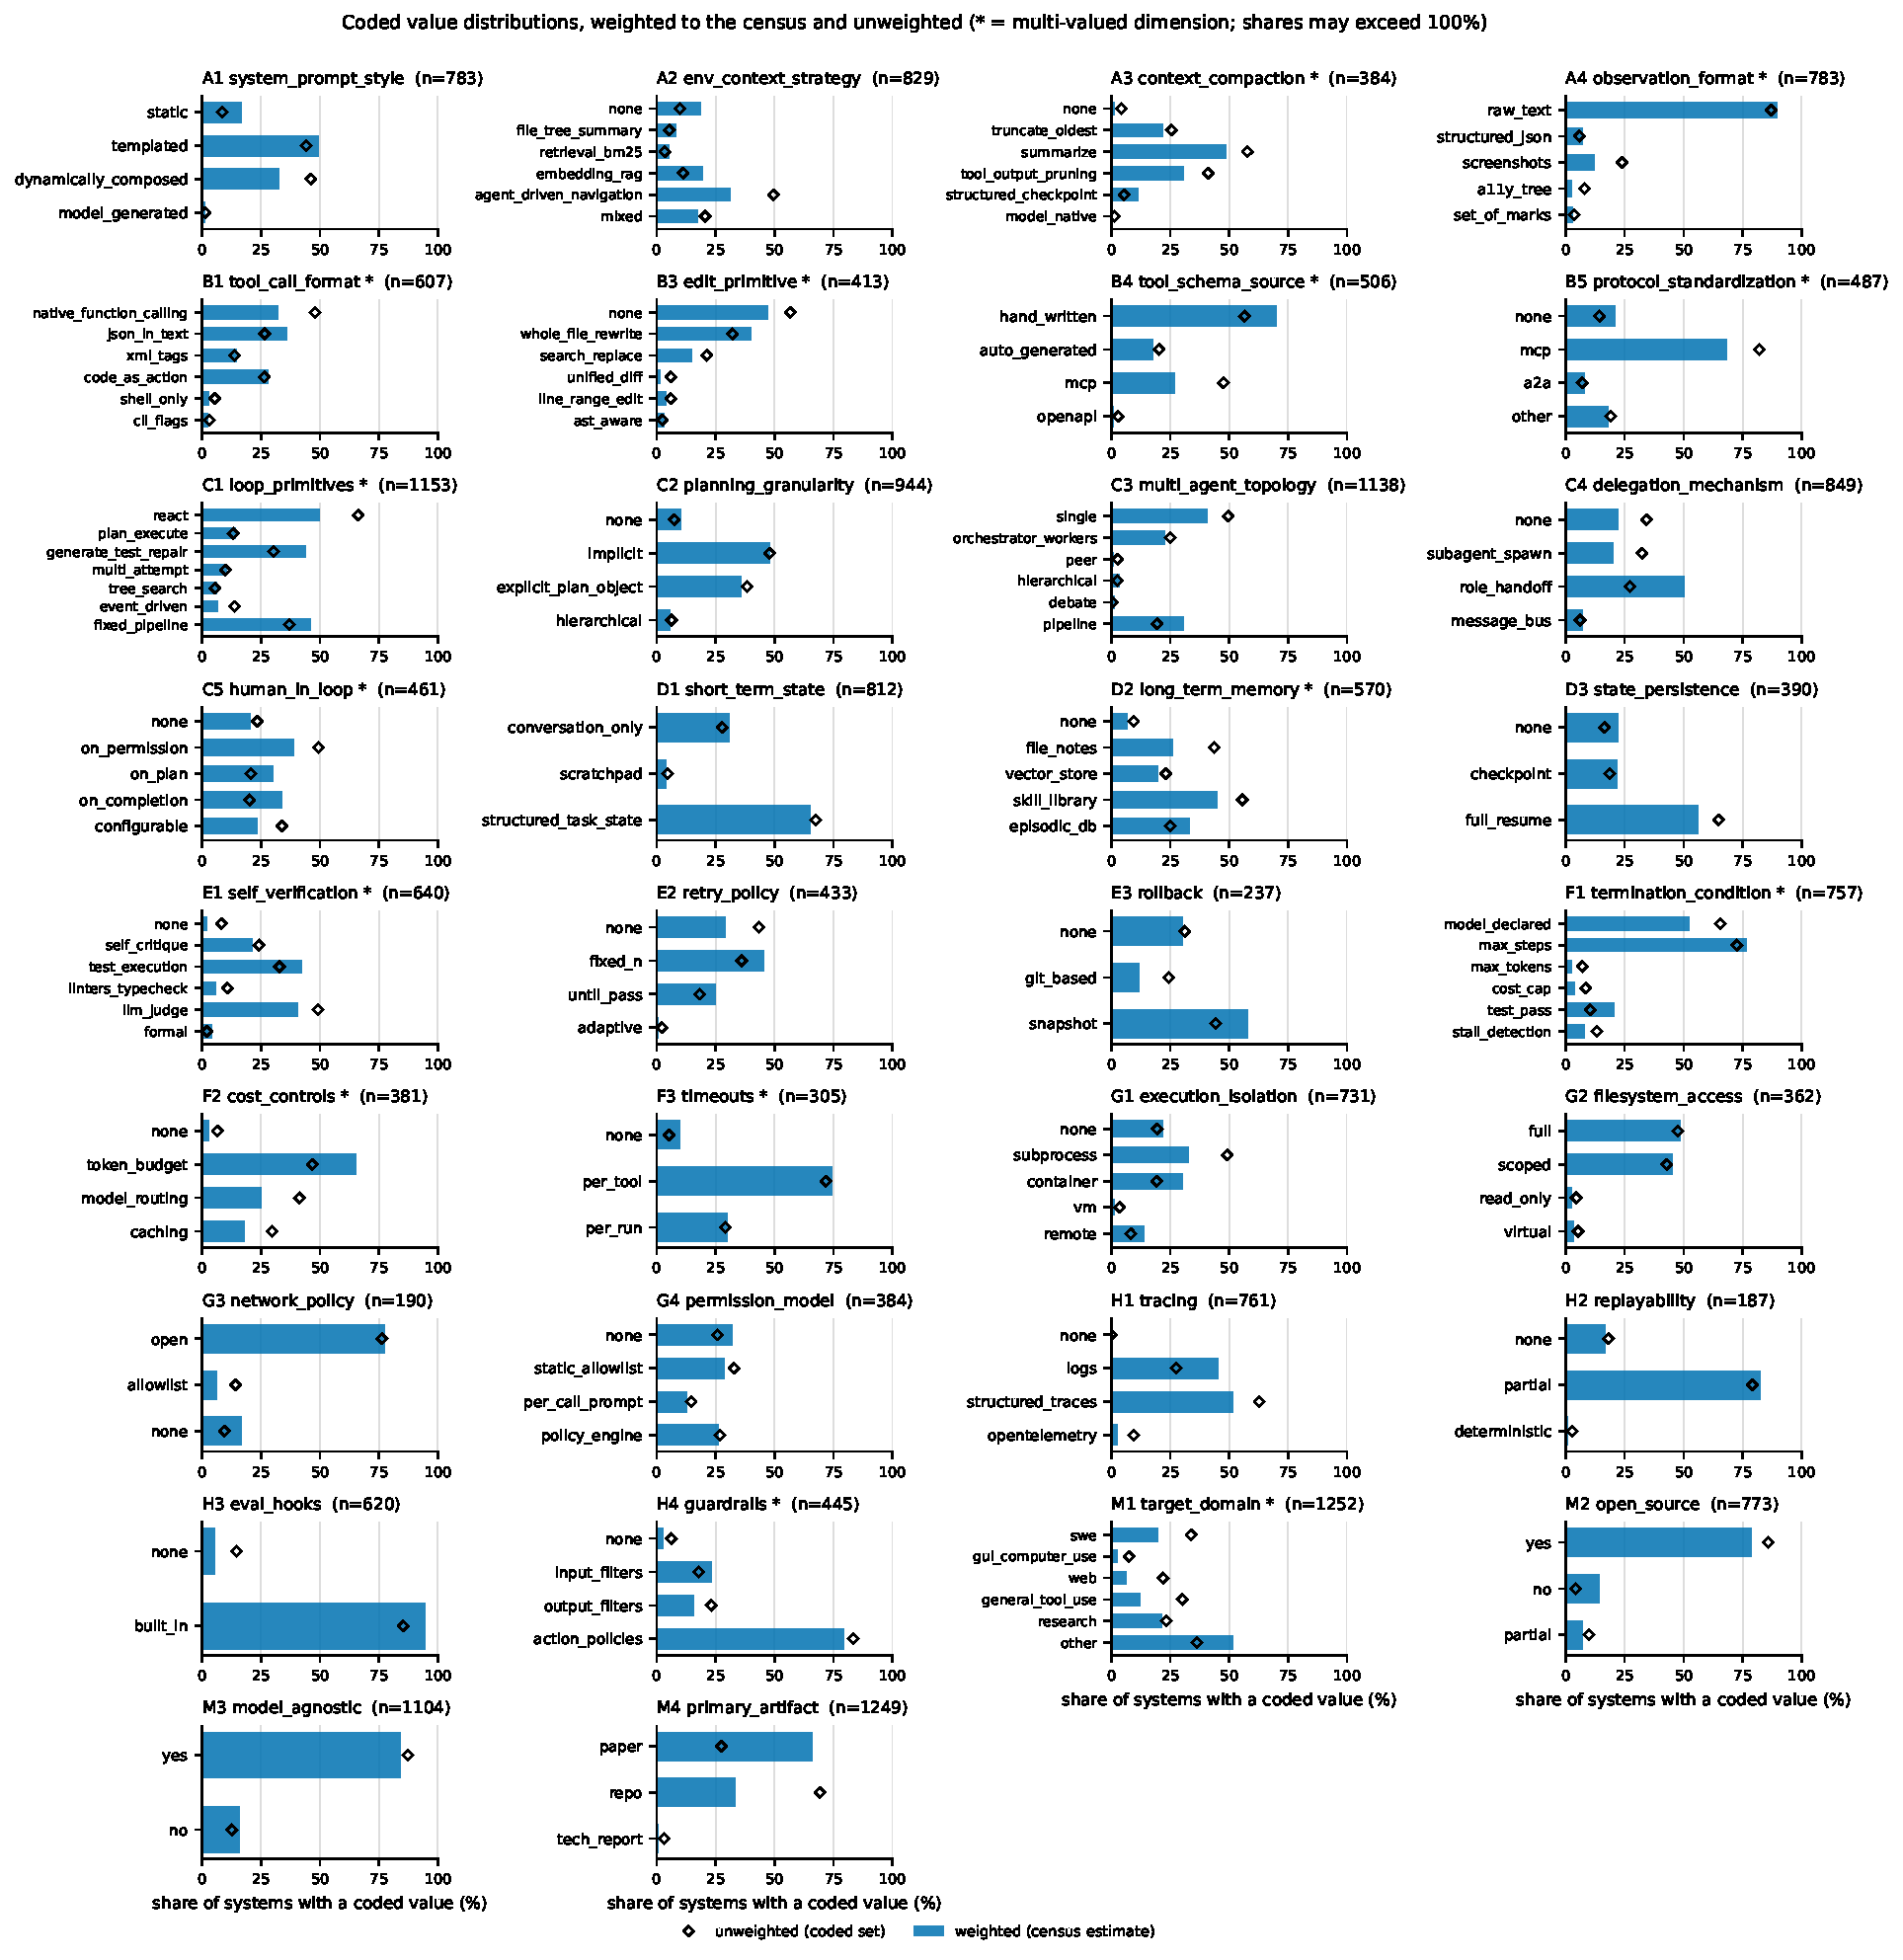
\includegraphics[width=\linewidth]{descriptives_value_distributions}
\caption{Weighted value distributions for every coded dimension, with the unweighted share of the coded
set marked on each bar. The gap between bar and marker is the sampling distortion for that value, and it
is largest for \texttt{primary\_artifact}, where the modal value changes.}
\label{fig:landscape_values}
\end{figure}

\subsection{Silence per dimension}
\label{subsec:moved-underreporting}

Figure~\ref{fig:landscape_underreporting} accompanies \S6.2 of the main paper, whose table gives
the silence rate by layer and for the five least-documented dimensions; the figure gives it for
every dimension, unweighted against weighted.

\begin{figure}[htbp]
\centering
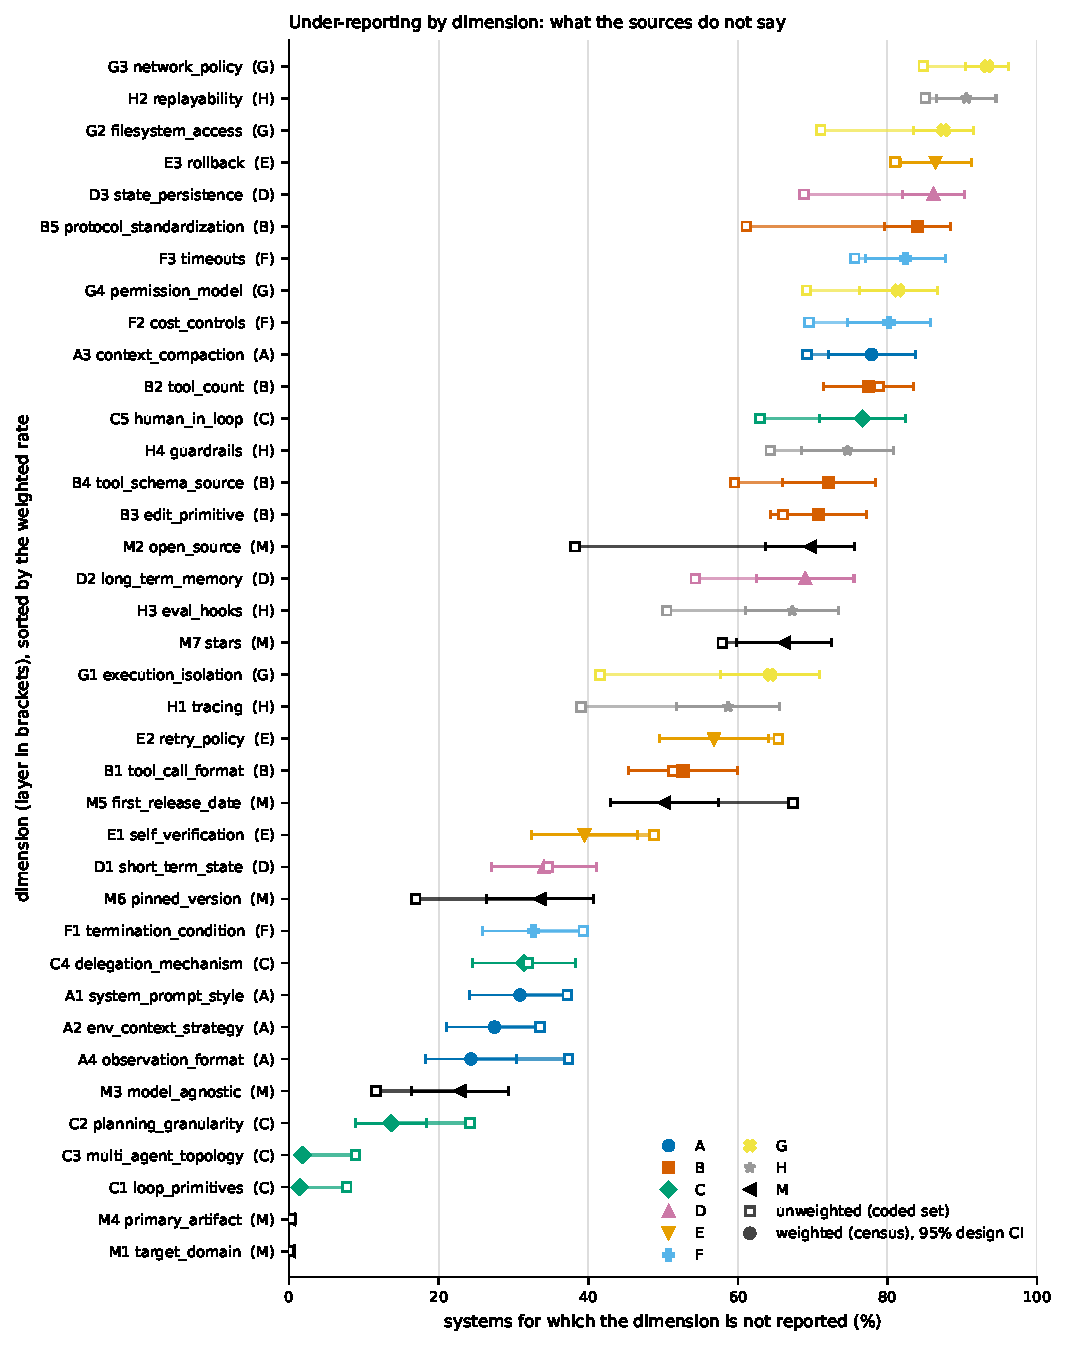
\includegraphics[width=0.9\linewidth]{descriptives_under_reporting_by_dimension}
\caption{Share of systems whose sources are silent, per dimension, unweighted against weighted. Weighting
raises the silence rate most for \texttt{open\_source}, \texttt{protocol\_standardization}, and
\texttt{execution\_isolation}, and lowers it for most control-loop dimensions. A review that codes only
visible systems understates the silence on what bounds an agent.}
\label{fig:landscape_underreporting}
\end{figure}

\subsection{Entropy trajectories}
\label{subsec:moved-trajectories}

Figure~\ref{fig:landscape_trajectories} accompanies \S6.3 of the main paper, whose table gives
the entropy change, interval and corrected $q$ for the ten dimensions whose interval excludes zero.

\begin{figure}[htbp]
\centering
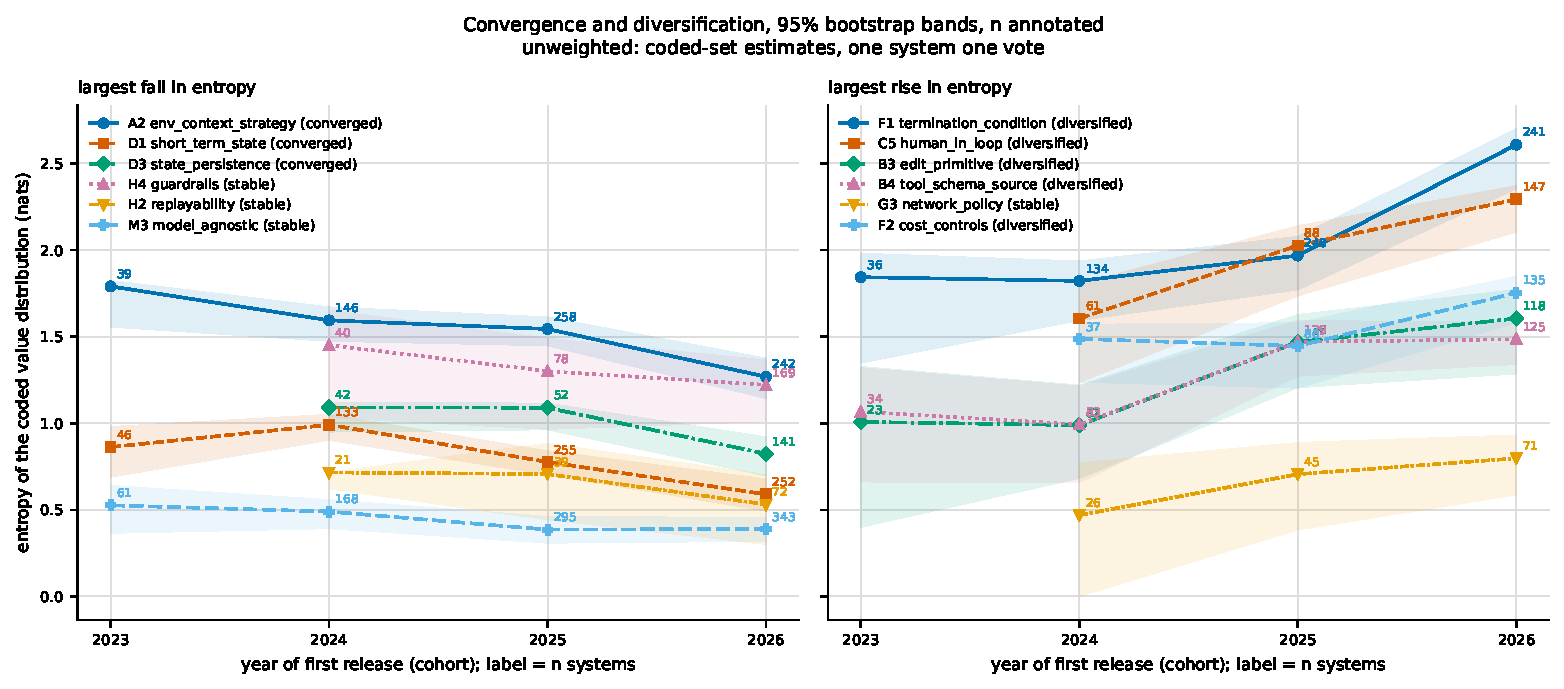
\includegraphics[width=\linewidth]{descriptives_entropy_trajectories}
\caption{The largest entropy falls and rises, with the number of reporting systems at each point. The
$n$ labels are why falls are read more cautiously than rises: a fall with rising $n$ can reflect who
reports rather than what is built. Unweighted; the legend's verdicts are uncorrected, and all six plotted
dimensions survive the Benjamini--Hochberg correction.}
\label{fig:landscape_trajectories}
\end{figure}

\subsection{Where shared silence creates association}
\label{subsec:moved-assoc}

Figure~\ref{fig:landscape_assoc_delta} accompanies \S6.5 of the main paper. It locates, pair by pair,
the change in association when \texttt{not\_reported} is counted as a level rather than excluded.

\begin{figure}[htbp]
\centering
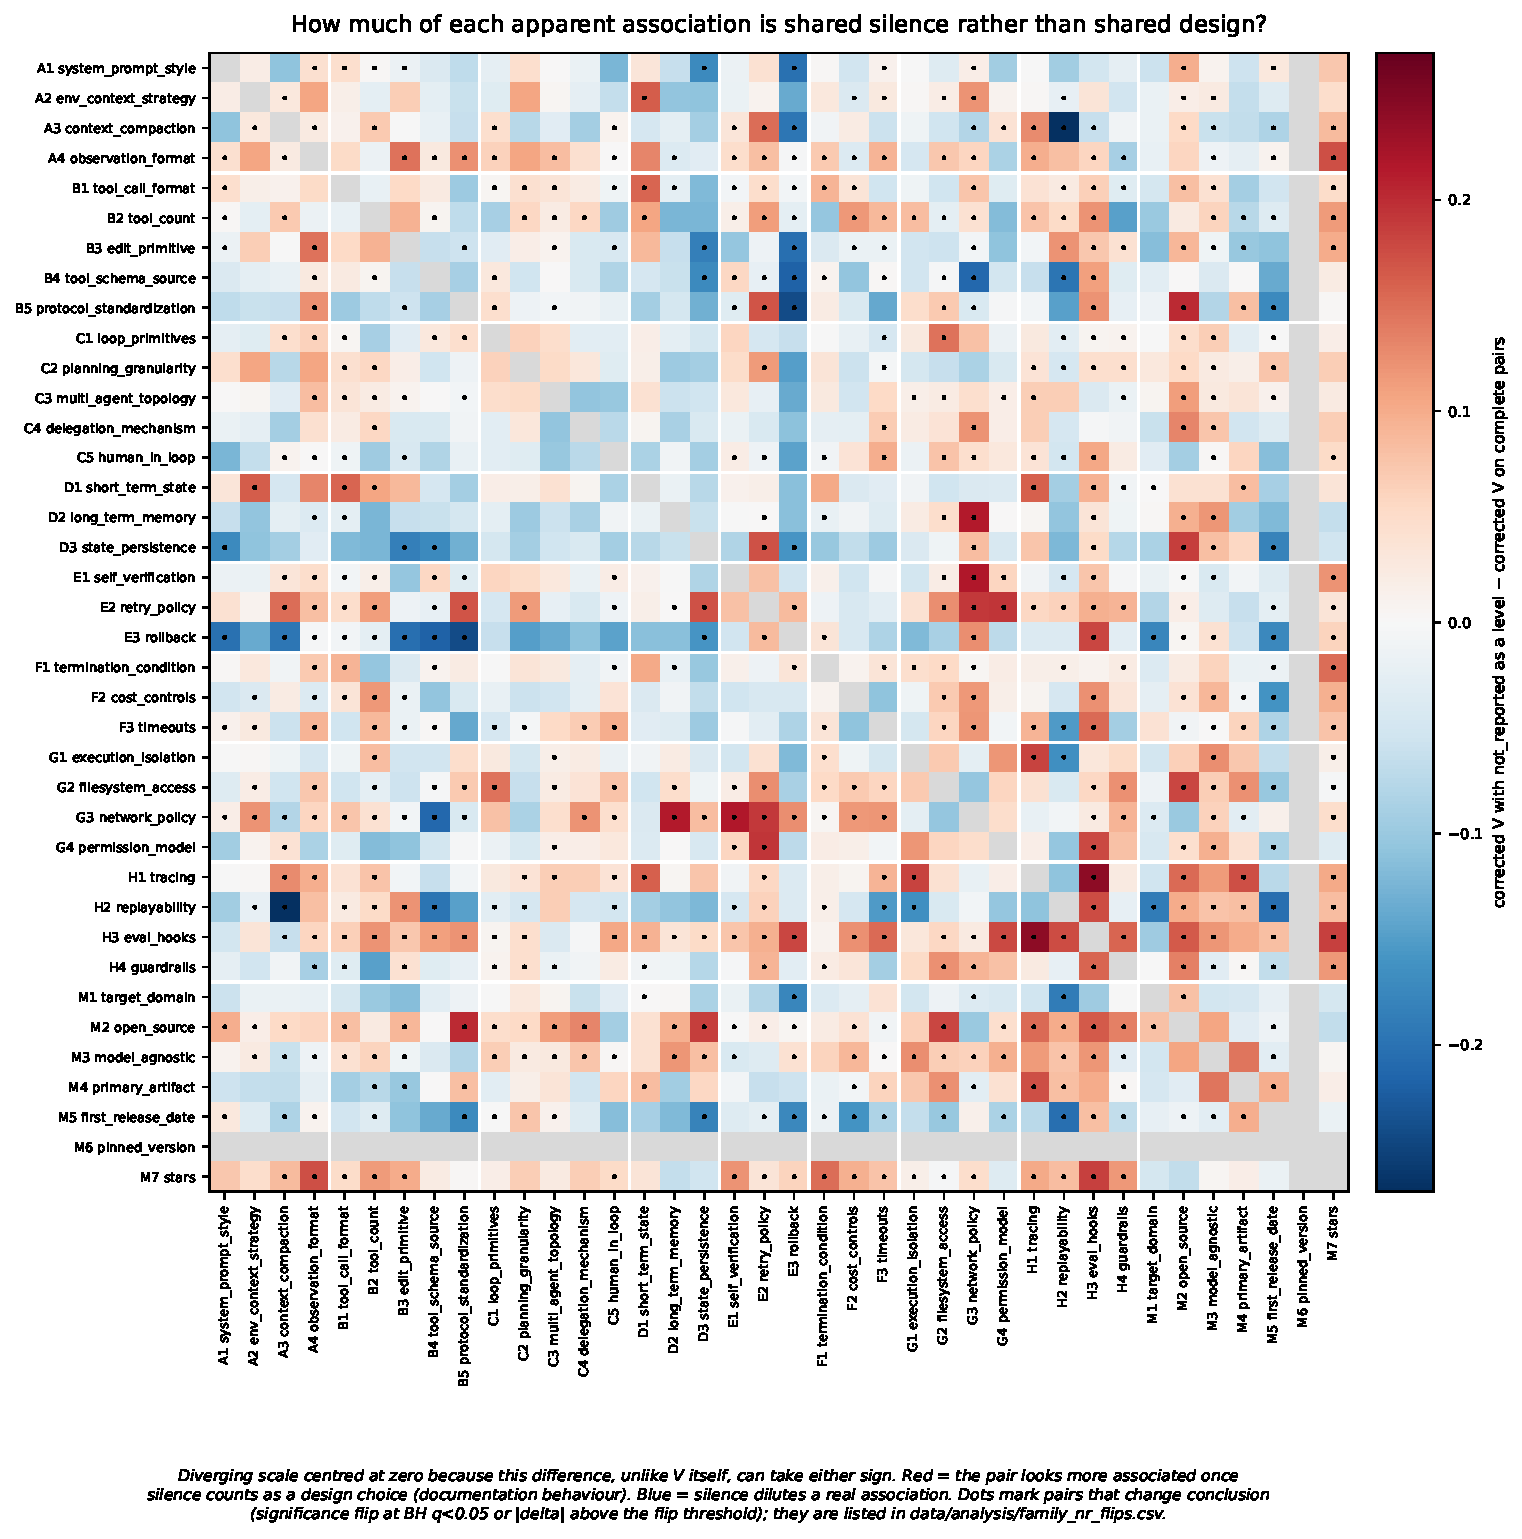
\includegraphics[width=\linewidth]{family_association_delta}
\caption{Corrected Cram\'er's V with \texttt{not\_reported} counted as a level minus the same coefficient
on complete pairs. Warm cells look more associated once silence is treated as a design choice; marked
cells change significance or move by at least 0.15. Most of the warmth is documentation habit, not design: 265 pairs
are significant only with silence as a level.}
\label{fig:landscape_assoc_delta}
\end{figure}


\bibliographystyle{ACM-Reference-Format}
\bibliography{references/must_cite}

\end{document}
